% Chapter 1

\chapter{Introducción general} % Main chapter title

\label{Chapter1} % For referencing the chapter elsewhere, use \ref{Chapter1} 
\label{IntroGeneral}

%----------------------------------------------------------------------------------------

% Define some commands to keep the formatting separated from the content 
\newcommand{\keyword}[1]{\textbf{#1}}
\newcommand{\tabhead}[1]{\textbf{#1}}
\newcommand{\code}[1]{\texttt{#1}}
\newcommand{\file}[1]{\texttt{\bfseries#1}}
\newcommand{\option}[1]{\texttt{\itshape#1}}
\newcommand{\grados}{$^{\circ}$}

%----------------------------------------------------------------------------------------

%\section{Introducción}

%----------------------------------------------------------------------------------------
\section{Descripción de la problemática}

La fenómica hace referencia a la obtención de un gran caudal de datos de las características de las plantas, lo que se denomina el fenotipo de la planta. Esta disciplina está en auge en la actualidad debido a sus aplicaciones potenciales. Por un lado, habilita el mejoramiento a gran escala debido a que es necesario vincular una gran cantidad de datos genéticos con datos fenotípicos para identificar la función de los genes. Por otro lado, si se incluyen otros conjuntos de datos como son los climáticos, permite realizar predicciones precisas sobre el comportamiento de las variedades, el cual es necesario para implementar lo que se conoce como agricultura de precisión. Sin embargo, la fruticultura no ha dado el salto hacia la fenómica.

En la  Estación Experimental Agropecuaria (EEA) de San Pedro se ha logrado secuenciar el ADN de más de 250 variedades de duraznero \cite{ARTICLE:1} disponiendo de una base de datos genómica de 75 gigabases (Gb) de ADN. Esta base permite identificar genes que controlan características del duraznero mediante algoritmos de inteligencia artificial (IA). Además, se dispone de datos climáticos diarios que se toman de forma automática que incluyen: las temperaturas medias, precipitaciones, horas de frío, radiación, etc. Esta información se combina con los datos genómicos y posteriormente, con modelos de IA se predice el comportamiento de las variedades en escenarios climáticos futuros.

En la actualidad, las heladas primaverales son el mayor problema de los frutales a nivel mundial. Este fenómeno ocurre cuando las flores abiertas se someten a temperaturas cercanas a los -2.5 °C. Por este motivo, es necesario conocer el número de flores que se encuentran en estado vulnerable ante un pronóstico de heladas primaverales, así también como la densidad de flores. Es del interés del Instituto Nacional de Tecnología Agropecuaria (INTA) determinar el estado fenológico a campo y mejorar para la tolerancia a heladas. En cuanto al mejoramiento, se ha realizado una caracterización a gran escala de la tolerancia a heladas de la colección de duraznero con el objetivo de identificar los genes responsables. Parte de ese experimento consistió en determinar en registrar el estado fenológico mediante fotos.

\section{Motivación}

Si sos nuevo en \LaTeX{}, hay un muy buen libro electrónico - disponible gratuitamente en Internet como un archivo PDF - llamado, \enquote{A (not so short) Introduction to \LaTeX{}}. El título del libro es generalmente acortado a simplemente \emph{lshort}. Puede descargar la versión más reciente en inglés (ya que se actualiza de vez en cuando) desde aquí:
\url{http://www.ctan.org/tex-archive/info/lshort/english/lshort.pdf}

Se puede encontrar la versión en español en la lista en esta página: \url{http://www.ctan.org/tex-archive/info/lshort/}

\subsubsection{Una subsubsección}

Acá tiene un ejemplo de una ``subsubsección'' que es el cuarto nivel de ordenamiento del texto, después de capítulo, sección y subsección.  Como se puede ver, las subsubsecciones no van numeradas en el cuerpo del documento ni en el índice.  El formato está definido por la plantilla y no debe ser modificado.

\subsection{Guía matemática rápida para \LaTeX{}}

Si estás escribiendo un documento con mucho contenido matemático, entonces es posible que desees leer el documento de la AMS (American Mathematical Society) llamado, \enquote{A Short Math Guide for \LaTeX{}}. Se puede encontrar en línea en el siguiente link: \url{http://www.ams.org/tex/amslatex.html} en la sección \enquote{Additional Documentation} hacia la parte inferior de la página.


%----------------------------------------------------------------------------------------

\section{Utilizando esta plantilla}

Si estás familiarizado con \LaTeX{}, entonces podés explorar la estructura de directorios de esta plantilla y proceder a personalizarla agregando tu información en el bloque \emph{INFORMACIÓN DE LA PORTADA} en el archivo \file{memoria.tex}.  

Se puede continuar luego modificando el resto de los archivos siguiendo los lineamientos que se describen en la sección \ref{sec:FillingFile} en la página \pageref{sec:FillingFile}.

Debés asegurarte de leer el capítulo \ref{Chapter2} acerca de las convenciones utilizadas para las Memoria de los Trabajos Finales de la \degreename.

Si sos nuevo en \LaTeX{}, se recomienda que continúes leyendo el documento ya que contiene información básica para aprovechar el potencial de esta herramienta.


%----------------------------------------------------------------------------------------

\section{Qué incluye esta plantilla}

\subsection{Carpetas}

Esta plantilla se distribuye como una único archivo .zip que se puede descomprimir en varios archivos y carpetas. Asimismo, se puede consultar el repositorio git para obtener la última versión de los archivos, \url{https://github.com/patriciobos/Plantilla-CESE.git}. Los nombres de las carpetas son, o pretender ser, auto-explicativos.

\keyword{Appendices} -- Esta es la carpeta donde se deben poner los apéndices. Cada apéndice debe ir en su propio archivo \file{.tex}. Se incluye un ejemplo y una plantilla en la carpeta.

\keyword{Chapters} -- Esta es la carpeta donde se deben poner los capítulos de la memoria. Cada capítulo debe ir un su propio archivo \file{.tex} por separado.  Se ofrece por defecto, la siguiente estructura de capítulos y se recomienda su utilización dentro de lo posible:

\begin{itemize}
\item Capítulo 1: Introducción general	
\item Capítulo 2: Introducción específica
\item Capítulo 3: Diseño e implementación
\item Capítulo 4: Ensayos y resultados
\item Capítulo 5: Conclusiones

\end{itemize}

Esta estructura de capítulos es la que se recomienda para las memorias de la especialización.

\keyword{Figures} -- Esta carpeta contiene todas las figuras de la memoria.  Estas son las versiones finales de las imágenes que van a ser incluidas en la memoria.  Pueden ser imágenes en formato \textit{raster}\footnote{\url{https://en.wikipedia.org/wiki/Raster_graphics}} como \file{.png}, \file{.jpg} o en formato vectoriales\footnote{\url{https://en.wikipedia.org/wiki/Vector_graphics}} como \file{.pdf}, \file{.ps}.  Se debe notar que utilizar imágenes vectoriales disminuye notablemente el peso del documento final y acelera el tiempo de compilación por lo que es recomendable su utilización siempre que sea posible.

\subsection{Archivos}

También están incluidos varios archivos, la mayoría de ellos son de texto plano y se puede ver su contenido en un editor de texto. Después de la compilación inicial, se verá que más archivos auxiliares son creados por \ LaTeX{} o BibTeX, pero son de uso interno y no es necesario hacer nada en particular con ellos.  Toda la información necesaria para compilar el documento se encuentra en los archivos \file{.tex}, \file{.bib}, \file{.cls} y en las imágenes de la carpeta Figures.

\keyword{referencias.bib} - este es un archivo importante que contiene toda la información de referencias bibliográficas que se utilizarán para las citas en la memoria en conjunto con BibTeX. Usted puede escribir las entradas bibliográficas en forma manual, aunque existen también programas de gestión de referencias que facilitan la creación y gestión de las referencias y permiten exportarlas en formato BibTeX.  También hay disponibles sitios web como \url{books.google.com} que permiten obtener toda la información necesaria para una cita en formato BibTeX. Ver sección \ref{sec:biblio}

\keyword{MastersDoctoralThesis.cls} -- este es un archivo importante. Es el archivos con la clase que le informa a \LaTeX{} cómo debe dar formato a la memoria. El usuario de la plantilla no debería necesitar modificar nada de este archivo.

\keyword{memoria.pdf} -- esta es su memoria con una tipografía bellamente compuesta (en formato de archivo PDF) creado por \LaTeX{}. Se distribuye con la plantilla y después de compilar por primera vez sin hacer ningún cambio se debería obtener una versión idéntica a este documento.

\keyword{memoria.tex} -- este es un archivo importante. Este es el archivo que tiene que compilar \LaTeX{} para producir la memoria como un archivo PDF. Contiene un marco de trabajo y estructuras que le indican a \LaTeX{} cómo diagramar la memoria.  Está altamente comentado para que se pueda entender qué es lo que realiza cada línea de código y por qué está incluida en ese lugar.  En este archivo se debe completar la información personalizada de las primeras sección según se indica en la sección \ref{sec:FillingFile}.

Archivos que \emph{no} forman parte de la distribución de la plantilla pero que son generados por \LaTeX{} como archivos auxiliares necesarios para la producción de la memoria.pdf son:

\keyword{memoria.aux} -- este es un archivo auxiliar generado por \LaTeX{}, si se borra \LaTeX{} simplemente lo regenera cuando se compila el archivo principal \file{memoria.tex}.

\keyword{memoria.bbl} -- este es un archivo auxiliar generado por BibTeX, si se borra BibTeX simplemente lo regenera cuando se compila el archivo principal \file{memoria.tex}. Mientras que el archivo \file{.bib} contiene todas las referencias que hay, este archivo \file{.bbl} contine sólo las referencias que han sido citadas y se utiliza para la construcción de la bibiografía.

\keyword{memoria.blg} -- este es un archivo auxiliar generado por BibTeX, si se borra BibTeX simplemente lo regenera cuando se compila el archivo principal \file{memoria.tex}.

\keyword{memoria.lof} -- este es un archivo auxiliar generado por \LaTeX{}, si se borra \LaTeX{} simplemente lo regenera cuando se compila el archivo principal \file{memoria.tex}.  Le indica a \LaTeX{} cómo construir la sección \emph{Lista de Figuras}.
 
\keyword{memoria.log} --  este es un archivo auxiliar generado por \LaTeX{}, si se borra \LaTeX{} simplemente lo regenera cuando se compila el archivo principal \file{memoria.tex}. Contiene mensajes de \LaTeX{}. Si se reciben errores o advertencias durante la compilación, se guardan en este archivo \file{.log}.

\keyword{memoria.lot} -- este es un archivo auxiliar generado por \LaTeX{}, si se borra \LaTeX{} simplemente lo regenera cuando se compila el archivo principal \file{memoria.tex}.  Le indica a \LaTeX{} cómo construir la sección \emph{Lista de Tablas}.

\keyword{memoria.out} -- este es un archivo auxiliar generado por \LaTeX{}, si se borra \LaTeX{} simplemente lo regenera cuando se compila el archivo principal \file{memoria.tex}.

De esta larga lista de archivos, sólo aquellos con la extensión \file{.bib}, \file{.cls} y \file{.tex} son importantes.  Los otros archivos auxiliares pueden ser ignorados o borrados ya que \LaTeX{} y BibTeX los regenerarán durante la compilación.

%----------------------------------------------------------------------------------------

\section{Entorno de trabajo}

Ante de comenzar a editar la plantilla debemos tener un editor \LaTeX{} instalado en nuestra computadora.  En forma análoga a lo que sucede en lenguaje C, que se puede crear y editar código con casi cualquier editor, existen ciertos entornos de trabajo que nos pueden simplificar mucho la tarea.  En este sentido, se recomienda, sobre todo para los principiantes en \LaTeX{} la utilización de TexMaker, un programa gratuito y multi-plantaforma que está disponible tanto para windows como para sistemas GNU/linux.

La versión más reciente de TexMaker es la 4.5 y se puede descargar del siguiente link: \url{http://www.xm1math.net/texmaker/download.html}. Se puede consultar el manual de usuario en el siguiente link: \url{http://www.xm1math.net/texmaker/doc.html}.
 

\subsection{Paquetes adicionales}

Si bien durante el proceso de instalación de TexMaker, o cualquier otro editor que se haya elegido, se instalarán en el sistema los paquetes básicos necesarios para trabajar con \LaTeX{}, la plantilla de los trabajos de Especialización y Maestría requieren de paquete adicionales.

Se indican a continuación los comandos que se deben introducir en la consola de Ubuntu (ctrl + alt + t) para instalarlos:

\begin{lstlisting}[language=bash]
  $ sudo apt install texlive-lang-spanish texlive-science 
  $ sudo apt install texlive-bibtex-extra biber
  $ sudo apt install texlive texlive-fonts-recommended
  $ sudo apt install texlive-latex-extra
\end{lstlisting}


\subsection{Configurando TexMaker}
\label{subsec:configurando}



Una vez instalado el programa y los paquetes adicionales se debe abrir el archivo memoria.tex con el editor para ver una pantalla similar a la que se puede apreciar en la figura \ref{fig:texmaker}. 
Una vez instalado el programa y los paquetes adicionales se debe abrir el archivo memoria.tex con el editor para ver una pantalla similar a la que se puede apreciar en la figura \ref{fig:texmaker}. 
Una vez instalado el programa y los paquetes adicionales se debe abrir el archivo memoria.tex con el editor para ver una pantalla similar a la que se puede apreciar en la figura \ref{fig:texmaker}. 
Una vez instalado el programa y los paquetes adicionales se debe abrir el archivo memoria.tex con el editor para ver una pantalla similar a la que se puede apreciar en la figura \ref{fig:texmaker}. 

\vspace{1cm}

\begin{figure}[htbp]
	\centering
	\includegraphics[width=.5\textwidth]{./Figures/texmaker.png}
	\caption{Entorno de trabajo de texMaker.}
	\label{fig:texmaker}
\end{figure}

\vspace{1cm}

Notar que existe una vista llamada Estructura a la izquierda de la interfaz que nos permite abrir desde dentro del programa los archivos individuales de los capítulos.  A la derecha se encuentra una vista con el archivo propiamente dicho para su edición. Hacia la parte inferior se encuentra una vista del log con información de los resultados de la compilación.  En esta última vista pueden aparecen advertencias o \textit{warning}, que normalmente pueden ser ignorados, y los errores que se indican en color rojo y deben resolverse para que se genere el PDF de salida.

Recordar que el archivo que se debe compilar con PDFLaTeX es \file{memoria.tex}, si se tratara de compilar alguno de los capítulos saldría un error.  Para salvar la molestia de tener que cambiar de archivo para compilar cada vez que se realice una modificación en un capítulo, se puede definir el archivo \file{memoria.tex} como ``documento maestro'' yendo al menú opciones -> ``definir documento actual como documento maestro'', lo que permite compilar con PDFLaTeX memoria.tex directamente desde cualquier archivo que se esté modificando . Se muestra esta opción en la figura \ref{fig:docMaestro}.

\begin{figure}[h]
	\centering
	\includegraphics[width=\textwidth]{./Figures/docMaestro.png}
	\caption{Definir memoria.tex como documento maestro.}
	\label{fig:docMaestro}
\end{figure}

En el menú herramientas se encuentran las opciones de compilación.  Para producir un archivo PDF a partir de un archivo .tex se debe ejecutar PDFLaTeX (el shortcut es F6). Para incorporar nueva bibliografía se debe utilizar la opción BibTeX del mismo menú herramientas (el shortcut es F11).

Notar que para actualizar las tablas de contenidos se debe ejecutar PDFLaTeX dos veces.  Esto se debe a que es necesario actualizar algunos archivos auxiliares antes de obtener el resultado final.  En forma similar, para actualizar las referencias bibliográficas se debe ejecutar primero PDFLaTeX, después BibTeX y finalmente PDFLaTeX dos veces por idénticos motivos.

\section{Personalizando la plantilla, el archivo \file{memoria.tex}}
\label{sec:FillingFile}

Para personalizar la plantilla se debe incorporar la información propia en los distintos archivos \file{.tex}. 

Primero abrir \file{memoria.tex} con TexMaker (o el editor de su preferencia). Se debe ubicar dentro del archivo el bloque de código titulado \emph{INFORMACIÓN DE LA PORTADA} donde se deben incorporar los primeros datos personales con los que se construirá automáticamente la portada.


%----------------------------------------------------------------------------------------

\section{El código del archivo \file{memoria.tex} explicado}

El archivo \file{memoria.tex} contiene la estructura del documento y es el archivo de mayor jerarquía de la memoria.  Podría ser equiparable a la función \emph{main()} de un programa en C, o mejor dicho al archivo fuente .c donde se encuentra definida la función main().

La estructura básica de cualquier documento de \LaTeX{} comienza con la definición de clase del documento, es seguida por un preámbulo donde se pueden agregar funcionalidades con el uso de \texttt{paquetes} (equiparables a bibliotecas de C), y finalmente, termina con el cuerpo del documento, donde irá el contenido de la memoria.

\lstset{%
  basicstyle=\small\ttfamily,
  language=[LaTeX]{TeX}
}

\begin{lstlisting}
\documentclass{article}  <- Definicion de clase
\usepackage{listings}	 <- Preambulo

\begin{document}	 <- Comienzo del contenido propio 
	Hello world!
\end{document}
\end{lstlisting}


El archivo \file{memoria.tex} se encuentra densamente comentado para explicar qué páginas, secciones y elementos de formato está creando el código \LaTeX{} en cada línea. El código está dividido en bloques con nombres en mayúsculas para que resulte evidente qué es lo que hace esa porción de código en particular. Inicialmente puede parecer que hay mucho código \LaTeX{}, pero es principalmente código para dar formato a la memoria por lo que no requiere intervención del usuario de la plantilla.  Sí se deben personalizar con su información los bloques indicados como:

\begin{itemize}
	\item Informacion de la memoria
	\item Resumen
	\item Agradecimientos
	\item Dedicatoria
\end{itemize}

El índice de contenidos, las listas de figura de tablas se generan en forma automática y no requieren intervención ni edición manual por parte del usuario de la plantilla. 

En la parte final del documento se encuentran los capítulos y los apéndices.  Por defecto se incluyen los 5 capítulos propuestos que se encuentran en la carpeta /Chapters. Cada capítulo se debe escribir en un archivo .tex separado y se debe poner en la carpeta \emph{Chapters} con el nombre \file{Chapter1}, \file{Chapter2}, etc\ldots El código para incluir capítulos desde archivos externos se muestra a continuación.

\begin{verbatim}
	% Chapter 1

\chapter{Introducción general} % Main chapter title

\label{Chapter1} % For referencing the chapter elsewhere, use \ref{Chapter1} 
\label{IntroGeneral}

%----------------------------------------------------------------------------------------

% Define some commands to keep the formatting separated from the content 
\newcommand{\keyword}[1]{\textbf{#1}}
\newcommand{\tabhead}[1]{\textbf{#1}}
\newcommand{\code}[1]{\texttt{#1}}
\newcommand{\file}[1]{\texttt{\bfseries#1}}
\newcommand{\option}[1]{\texttt{\itshape#1}}
\newcommand{\grados}{$^{\circ}$}

%----------------------------------------------------------------------------------------

%\section{Introducción}

%----------------------------------------------------------------------------------------

En este capítulo se presenta la problemática y la motivación que llevaron a la realización del presente trabajo.

\section{Descripción de la problemática}

La fenómica hace referencia a la obtención de un gran caudal de datos de las características de las plantas, lo que se denomina el fenotipo de la planta. Esta disciplina está en auge en la actualidad debido a sus aplicaciones potenciales. Por un lado, habilita el mejoramiento a gran escala debido a que es necesario vincular una gran cantidad de datos genéticos con datos fenotípicos para identificar la función de los genes. Por otro lado, si se incluyen otros conjuntos de datos como son los climáticos, permite realizar predicciones precisas sobre el comportamiento de las variedades, el cual es necesario para implementar lo que se conoce como agricultura de precisión. Sin embargo, la fruticultura no ha dado el salto hacia la fenómica.

En la  Estación Experimental Agropecuaria (EEA) de San Pedro se ha logrado secuenciar el ADN de más de 250 variedades de duraznero \cite{ARTICLE:1} disponiendo de una base de datos genómica de 75 gigabases (Gb) de ADN. Esta base permite identificar genes que controlan características del duraznero mediante algoritmos de inteligencia artificial (IA). Además, se dispone de datos climáticos diarios que se toman de forma automática que incluyen: las temperaturas medias, precipitaciones, horas de frío, radiación, etc. Esta información se combina con los datos genómicos y posteriormente, con modelos de IA se predice el comportamiento de las variedades en escenarios climáticos futuros.

En la actualidad, las heladas primaverales son el mayor problema de los frutales a nivel mundial. Este fenómeno ocurre cuando las flores abiertas se someten a temperaturas cercanas a los -2.5 °C. Las heladas primaverales, tienen una temparatura parecida a cualquier otra helada que se puede presentar en la temporada de invierno. Sin embargo, estas heladas suelen presentarse despues del invierno, creando un gran impacto contra las flores y los frutos de los frutales. Los productores de frutas en general, se ven altamente afectados pagando un alto precio por estas inesperadas heladas tardías. En la figura \ref{fig:helada}, se puede observar como este fenomeno meteorológico afecta a los frutales.

\begin{figure}[htpb]
	\centering
	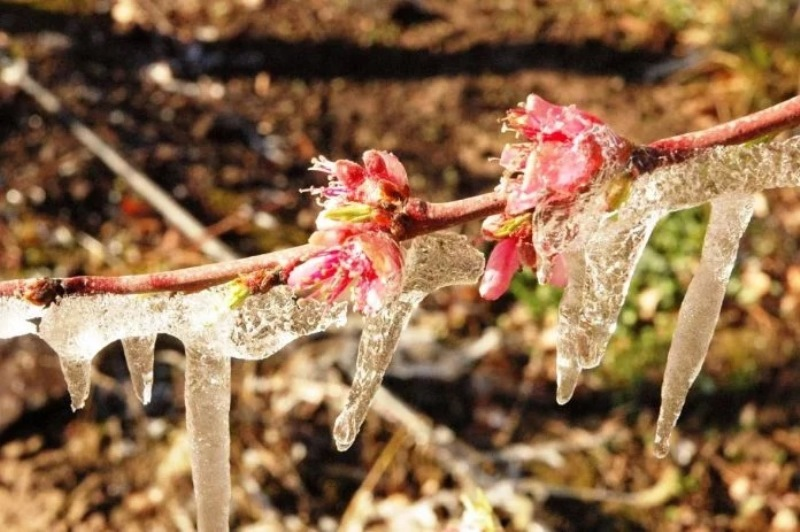
\includegraphics[scale=.5]{./Figures/heladas3.jpeg}
	\caption{Frutales afectados por las heladas primaverales \cite{WEBSITE:1}.}
	\label{fig:helada}
\end{figure}

\section{Motivación}

Por este motivo, es del interés del Instituto Nacional de Tecnología Agropecuaria (INTA) determinar el estado fenológico a campo y mejorar para la tolerancia a heladas.

Para determinar el estado fenológico a campo, es necesario conocer el número de flores que se encuentran en estado vulnerable ante un pronóstico de heladas primaverales, así también como la densidad de flores.

En cuanto al mejoramiento, se ha realizado una caracterización a gran escala de la tolerancia a heladas de la colección de duraznero con el objetivo de identificar los genes responsables. Parte de ese experimento consistió en determinar en registrar el estado fenológico mediante fotos.

El presente trabajo permitirá automatizar la toma de datos de varetas de duraznero, a partir de fotos para aumentar el caudal de datos y mejorar los modelos de IA.

\section{Requerimientos}

\begin{enumerate}
	\item Requerimientos funcionales
		\begin{enumerate}
			\item El sistema tomará como entrada imágenes de varetas de durazneros en formato JPG.			
			\item El algoritmo debe detectar la presencia de las varetas de los durazneros e identificar el tipo de flor que posee.			        
			\item El algoritmo debe identificar el estado fenológico de cada flor de duraznero en la vareta. Este estado se clasificará como  \textit{flor abierta}, \textit{flor cerrada}, \textit{flor sinpetalos}, \textit{incierto}.
			\item El algoritmo debe determinar la cantidad de flores por centímetro de vareta.
			\item El sistema debe entregar como resultado un archivo en formato CSV con los datos detectados por el algoritmo y una imagen donde se puedan visualizar las detecciones.
			\item El sistema debe funcionar en una computadora local.
		\end{enumerate}
	\item Requerimientos de diseño e implementación
		\begin{enumerate}
			\item El diseño debe ser modular.
			\item El algoritmo se elaborará en una notebook de Google Colab, utilizando el lenguaje de  programación Python y bibliotecas de IA correspondientes. 
		\end{enumerate}
	\item Requerimiento de evaluación y prueba
	\begin{enumerate}
			\item El modelo se evaluará con imágenes provenientes del mismo dataset de imágenes entregado por el cliente.
			 \item La métrica que se utilizará para la evaluación del modelo de detección será \textit{mean average precision} (mAP) y para el clasificador se tomarán en cuenta las métricas \textit{accuracy}, \textit{precision} y \textit{recall}.
		\end{enumerate}
	\item Requerimientos de documentación
	\begin{enumerate}
			\item El funcionamiento del sistema debe estar correctamente explicado y documentado.
			 \item El código estará correctamente comentado como parte de buenas prácticas del desarrollo de software.
			 \item Inclusión de documentación en un repositorio, mediante un archivo README.md (opcional).
		\end{enumerate}
\end{enumerate}

\section{Objetivo y alcances}

El objetivo de este trabajo es desarrollar un algoritmo que permita automatizar la toma de datos de las flores de duraznero a través de fotos de varetas.

El presente trabajo incluye:
\begin{itemize}
	\item El preprocesamiento de las fotos para entrenar el modelo.
	\item La selección del modelo a entrenar.
	\item La elaboración del notebook de pruebas en Python.
	\item La implementación local del modelo.
\end{itemize}

El trabajo no incluye:
\begin{itemize}
	\item La recolección de datos/fotos.
	\item La integración con otros modelos que utilice el cliente.
\end{itemize}


%----------------------------------------------------------------------------------------

\section{Estado del arte}

El presente trabajo contiene distintos algoritmos que integrados logran tomar los datos deseados. Es por este motivo, que para determinar el estado del arte es necesario desglosar cada algoritmo y evaluarlo individualmente como se hace acontinuación.

\subsection{Medición de la vareta}

En la actualidad, se han desarrollado algoritmos que pueden determinar el tamaño de distintos objetos a través de imágenes usando visión por computadora, muchos parten de encontrar un objeto de referencia al cual se le conocen sus dimensiones (alto y ancho). Este objeto de referencia, normalmente se selecciona por ser fácil de detectar, por conocer sus dimensiones y por ser un objeto único. El procedimiento habitual para su detección, es pasar la imagen a escala de grises, aplicar filtros gaussianos para eliminar el ruido, utilizar detección de bordes y por ultimo utilizar detección de contornos, tal y como se realiza en el trabajo \textbf{Measuring Size of an Object using Computer Vision} \cite{ARTICLE:2}. Cabe destacar que usualmente el fondo es de un color blanco facilitando la detección.

En el presente trabajo se tienen imágenes con fondos de color naranja en su mayoría, el objeto de refencia a veces se encuentra ocluido, las imágenes se encuentran en horizontal o vertical, el objeto de referencia no simpre tiene la misma posición, etc. Por estos motivos, se utilizó un metodo de detección más complejo con un modelo de detección de objetos que se conoce como \textit{YOLOv8} y se concidera el estado del arte a la fecha.

\subsection{Detección de los estados fenológicos de la flor de duraznero}
 
La detección de flores a sido estudiada con diferentes enfoques y arquitecturas de \textit{deep learning}, como por ejemplo \cite{ARTICLE:3} que exploró la viabilidad de detección de estados fenológico de las rosas con técnicas del contraste del color y comparando con el modelo de detección \textit{Faster-RCNN}. Sin embargo, no utilizo ninguna arquitectura de una etapa para la detección, lo cual podría ser más eficiente. Por otro lado, se tienen trabajos que si utilizaron la arquitectura de una etapa, en especifico de \textit{YOLO} en sus versiones 4 y 5 como se presenta en \cite{ARTICLE:4} \cite{ARTICLE:5}, pero su enfoque fue basado para las flores de kiwi.

El presente trabajo, busca en especifico los estado fenológicos de la flor de duraznero utilizando y comparando dos modelos de detección, uno que tiene una arquitectura de dos etapas y otro que tiene una arquitectura de una etapa. Con esto, se hace uso de \textit{YOLO} en su version 8 para la realización efectiva y eficiente de esta tarea, el cual representa el estado del arte en la actualidad.

\subsection{Conteo de flores}






%----------------------------------------------------------------------------------------


	\chapter{Introducción específica} % Main chapter title

\label{Chapter2}

%----------------------------------------------------------------------------------------
%	SECTION 1
%----------------------------------------------------------------------------------------
En este capítulo se presenta una introducción teórica detallada de los algoritmos utilizados para la elaboración del presente trabajo.

\section{Red neuronal convolucional}

Una red neuronal convolucional es un tipo red neuronal diseñada para identificar patrones en imágenes. Particularmente esta arquitectura de \textit{deep learning}, suele ser utilizada en problemas de visión por computadora relacionados a la clasificación o detección de objetos en una imagen. Estas redes, pueden llegar a tener cientos de capas y llegan a estar compuestas por tres tipos principales como son las capas convolucionales, las capas de agrupación (\textit{pooling}) y una o varias capas totalmente conectadas (\textit{fully connected}) \cite{WEBSITE:2}\cite{WEBSITE:3}\cite{WEBSITE:4}.

La capa convolucional consiste en un conjunto de filtros o \textit{kernels} entrenables que se mueven por el ancho y alto de la imagen de entrada, donde, se calcula el producto escalar entre los píxeles de entrada y el filtro en cualquier posición. El resultado de este calculo se incorpora en una matriz de salida. De esta forma, se desplaza el filtro repitiendo la operación anterior hasta que el \textit{kernel} recorre toda la imagen. La serie de productos escalares de la imagen de entrada con los filtros se conoce como mapa de activación. Finalmente, la red aprenderá filtros que se activan cuando detectan algún tipo de característica, borde o patrón visual \cite{WEBSITE:3}\cite{WEBSITE:4}.

La capa de agrupación, se encuentra normalmente entre capas sucesivas convolucionales. Su función es simplificar la salida mediante la reducción no lineal de la tasa de muestreo, lo que termina resultando en una disminución de la cantidad de parámetros que la red debe aprender. Aunque se pierde información en está capa, tiene beneficios para la red convolucional, como por ejemplo se reduce complejidad, mejora la eficiencia y evita el sobreajuste \cite{WEBSITE:3}\cite{WEBSITE:4}.

La capa totalmente conectada a diferencia de las otras capas mencionadas, es que tiene todos los nodos de la salida conectados directamente a los nodos anteriores. El objetivo de esta ultima capa, es realizar una clasificación, basándose en las características extraídas anteriormente. La función de activación generalmente utilizada en esta capa es la función \textit{softmax} para obtener la probabilidad de que un objeto pertenezca a una clase u otra entre un intervalo de 0 a 1.

En la figura \ref{fig:cnn}, se puede observar un ejemplo de como se estructuran dichas capas en la red neuronal convolucional.


\begin{figure}[ht]
	\centering
	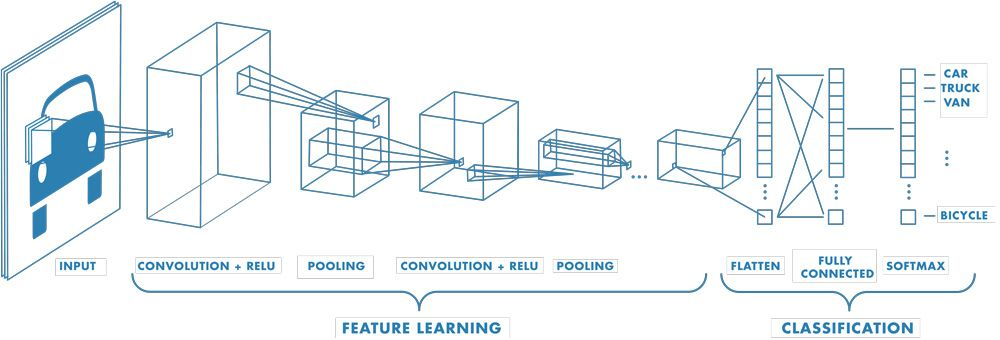
\includegraphics[scale=.45]{./Figures/cnn-image.jpeg}
	\caption{Ejemplo de arquitectura de red neuronal convolucional \cite{WEBSITE:2}.}
	\label{fig:cnn}
\end{figure}


\section{Detección de objetos}

La detección de objetos es una técnica utilizada en visión por computadora para localizar e identificar uno o varios objetos en una imagen o vídeo. A diferencia de otras técnicas de \textit{machine learning}, como es el caso de la clasificación o reconocimiento de imágenes, la detección busca localizar el lugar exacto donde se encuentra el objeto de interés y lo delimita con un rectángulo también llamado caja delimitadora o \textit{bounding box} por su termino en ingles. Por otro lado, una vez delimitado el objeto se clasifica entre las categorías disponibles \cite{WEBSITE:5}.

La detección de objetos se puede implementar utilizando métodos de \textit{machine learning} clásicos o de \textit{deep learning} dependiendo del problema a resolver\cite{WEBSITE:6}. El uso de \textit{deep learning} es más eficaz cuando se requiere tratar imágenes con muchas etiquetas, es decir, muchos objetos a detectar y las imágenes tienen otras variaciones como cambio de brillo, rotaciones, cambio de escala, etc. Por otro lado, el uso de \textit{machine learning} clásico es favorable cuando no se tienen altas capacidades de procesamiento y el número de etiquetas distintas a identificar es menor.

Algunos ejemplos de detección de objetos con \textit{machine learning} clásico son \textit{SIFT}, \textit{Temple Matching}, etc. En la figura \ref{fig:tempMatch}, se puede observar el uso de \textit{Temple Matching} para detectar el logo de Coca-Cola en una imagen.

\begin{figure}[ht]
	\centering
	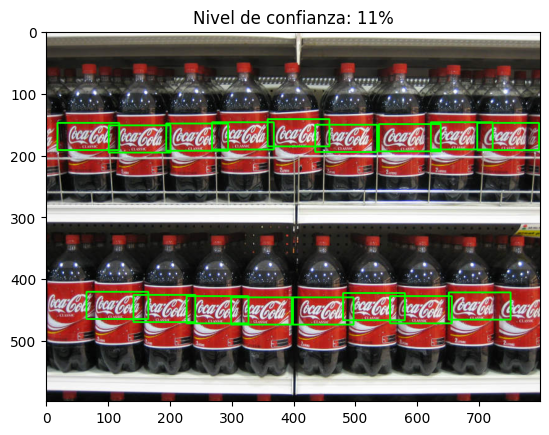
\includegraphics[scale=.45]{./Figures/template_match.png}
	\caption{Ejemplo de \textit{template matching} para identificar el logo de Coca-Cola.}
	\label{fig:tempMatch}
\end{figure}

Por otro lado, se tienen métodos de \textit{deep learning} para detección de objetos más avanzados que involucran detectores de dos etapas y de una etapa como son \textit{R-CNN}, \textit{Faster R-CNN}, \textit{SSD}, \textit{YOLO}, entre otros.

\subsection{Detectores de dos etapas}

Los detectores de dos etapas, como \textit{R-CNN} y sus variantes, primero extraen las características de la imagen y se propone la región de interés (ROI). El ROI, consiste en un \textit{bounding box} donde se presume que se encuentra el objeto a buscar. Luego, en la segunda etapa, se analiza las características encontradas en conjunto con el ROI, para seleccionar los \textit{bounding boxes} finales y calcular las probabilidades de que el objeto en las regiones pertenezca a una clase especifica \cite{ARTICLE:8}. 

Las redes neuronales de dos etapas son muy precisas al momento de detectar un objeto, sin embargo, son redes que son consideradas lentas durante la inferencia. Esta desventaja llevo a mejorar los modelos iniciales como \textit{R-CNN} a sus variantes \textit{Fast R-CNN} y \textit{Faster R-CNN}.

En la figura \ref{fig:rcnn}, se puede observar la arquitectura de una red neuronal de dos etapas \textit{R-CNN}.

\begin{figure}[ht]
	\centering
	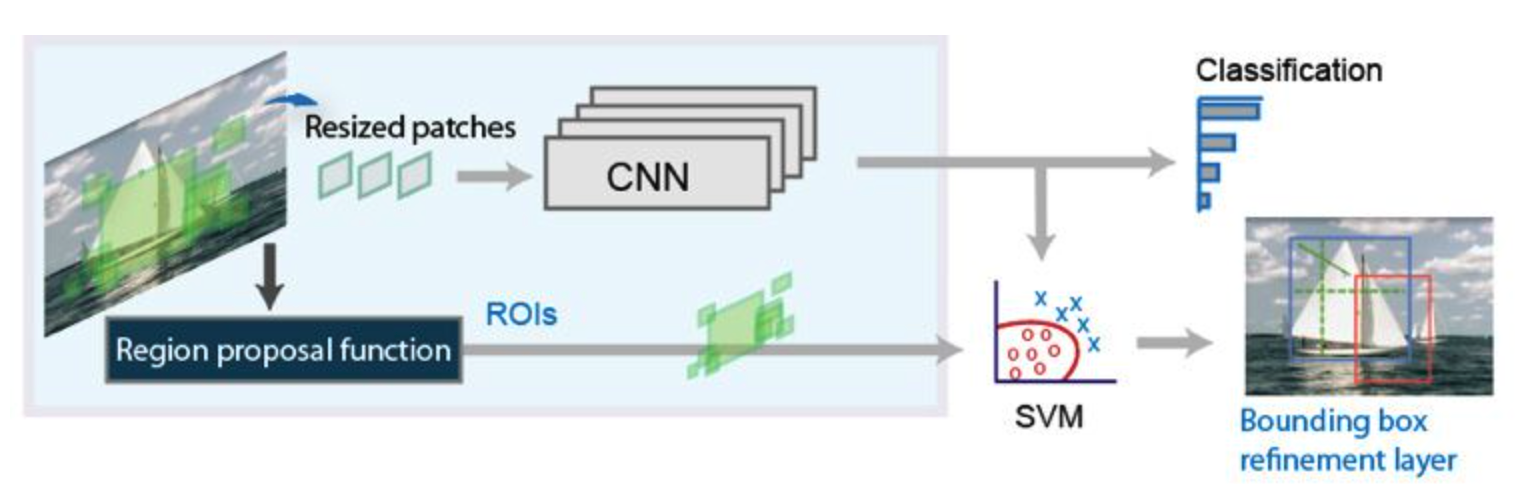
\includegraphics[scale=.25]{./Figures/R-CNN.png}
	\caption{Ejemplo de arquitectura de red neuronal de dos etapas \textit{R-CNN} \cite{WEBSITE:6}.}
	\label{fig:rcnn}
\end{figure}

\subsubsection{Detección de objetos con \textit{Fast R-CNN}}

Las mejoras adicionadas en \textit{Fast R-CNN} en comparación con \textit{R-CNN} incluyen una nueva capa llamada \textit{ROI Pooling}, que se encarga de extraer vectores de características de igual longitud de todas las regiones de interés propuestas. Por otro lado, \textit{R-CNN} contiene tres etapas como son la generación de región propuesta, la extracción de características y la clasificación usando \textit{SVM}, sin embargo, \textit{Fast R-CNN} crea una red neuronal que tiene una única etapa reduciendo así el número de etapas de su predecesor. Además, este modelo comparte cálculos computacionales a través de todas las ROIs propuestas en vez de hacerlo una a una de manera independiente. Por ultimo, \textit{Fast R-CNN} no guarda en cache las características, lo que reduce el uso de disco de memoria \cite{ARTICLE:10}.

\subsubsection{Detección de objetos con \textit{Faster R-CNN}}

El modelo \textit{Faster R-CNN} fue diseñado para superar muchos de los errores encontrados en sus predecesores como \textit{Fast R-CNN} y \textit{R-CNN}, en general como su nombre en ingles sugiere, sus mejoras van relacionadas a la rapidez en comparación a las otras variantes.

\textit{Faster R-CNN} mejora con respecto a \textit{Fast R-CNN} incorporando la red de región propuesta o por sus siglas en ingles RPN, que es una red completamente convolucional que produce propuestas con diferentes escalas y relaciones de aspecto. La RPN aplica la terminologia de redes neuronales con atención para indicar al modelo a donde mirar.

En \textit{Faster R-CNN} se introduce el concepto de \textit{anchor boxes}, lo que permite detectar objetos en distintas escalas y relaciones de aspecto. Por ultimo, se comparten cálculos computacionales a través la RPN y \textit{Fast R-CNN}, lo que reduce el tiempo computacional \cite{ARTICLE:9}. En la figura \ref{fig:Faster-rcnn}, se muestra un ejemplo de la arquitectura de \textit{Faster R-CNN}.

\begin{figure}[ht]
	\centering
	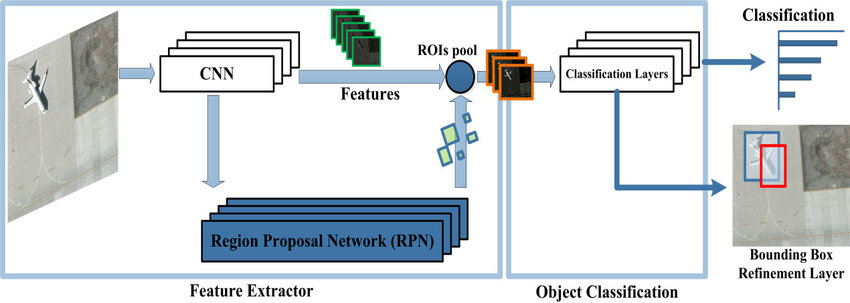
\includegraphics[scale=1.3]{./Figures/Faster-rcnn.png}
	\caption{Ejemplo de arquitectura de red neuronal de dos etapas \textit{Faster R-CNN} \cite{ARTICLE:11}.}
	\label{fig:Faster-rcnn}
\end{figure}

\subsection{Detectores de una etapa}

Los detectores de una etapa son modelos que omiten la etapa de RPN y ejecutan la detección directamente en un muestreo denso de ubicaciones. Estos modelos hacen uso de \textit{grid-box} y \textit{anchor box} para localizar la región de detección y delimitar al objeto de interés. En general, se consideran más rápidos que los detectores de dos etapas, sin embargo, son menos precisos \cite{ARTICLE:12}.

Algunos ejemplos de detectores de una etapa son las arquitecturas \textit{YOLO}, \textit{SSD}, \textit{RetinaNet}, \textit{SqueezeDet} y \textit{DetectNet}. 

\subsubsection{Detección de objetos con \textit{YOLO}}

\textit{You Only Look Once} (\textit{YOLO}) es considerado el estado del arte para la detección en tiempo real y fue introducido en el año 2015. En el paper \cite{ARTICLE:13}, los autores trataron la detección de objetos como un problema de regresión simple en vez de hacerlo como un problema de clasificación, donde se separa espacialmente los \textit{bounding boxes} y se les asocia una probabilidad a cada detección en la imagen usando una red neuronal convolucional.

El modelo funciona basado en el uso de bloques residuales, \textit{bounding boxes} por regresión, \textit{Intersection Over Unions} (\textit{IoU}) y \textit{Non-Maximum Suppression}.

El primer paso es el uso de bloques residuales que consiste en dividir la imagen original en celdas cuadriculadas de NxN de igual dimensión. Cada celda en la cuadricula es responsable de localizar y predecir la clase de objeto que cubre con su respectivo valor de confianza. Luego, se determinan los \textit{bounding boxes} con los atributos que \textit{YOLO} obtiene usando un modulo de regresión lineal. La respuesta que se recibe de este modulo es una representación vectorial de las coordenadas para cada \textit{bounding boxes}.

Por otro lado, un mismo objeto puede tener múltiples cuadriculas candidatas en la predicción, donde, no todas son relevantes. \textit{IoU} ayuda a descartar aquellas predicciones no relevantes dándole un valor entre 0 y 1 a cada una. Para esto, \textit{IoU} establece un umbral y posteriormente \textit{YOLO} calcula para cada cuadricula el \textit{IoU} y si es menor al umbral establecido, descarta dicha predicción. Por ultimo, se aplica \textit{Non-Maximum Suppression} para preservar solo aquellas predicciones que tengan un valor de confianza alto \cite{WEBSITE:7}.

\textit{YOLO} ha tenido muchas versiones donde se ha ido mejorando la velocidad, la precisión, el uso de recursos, entre otros. Estas versiones van desde la uno a la nueve. Siendo la ocho la usada en la presente memoria.

\section{Clasificación de objetos}



%\subsection{Uso de mayúscula inicial para los título de secciones}
%
%Si en el texto se hace alusión a diferentes partes del trabajo referirse a ellas como capítulo, sección o subsección según corresponda. Por ejemplo: ``En el capítulo \ref{Chapter1} se explica tal cosa'', o ``En la sección \ref{sec:ejemplo} se presenta lo que sea'', o ``En la subsección \ref{subsec:ejemplo} se discute otra cosa''.
%
%Cuando se quiere poner una lista tabulada, se hace así:
%
%\begin{itemize}
%	\item Este es el primer elemento de la lista.
%	\item Este es el segundo elemento de la lista.
%\end{itemize}
%
%Notar el uso de las mayúsculas y el punto al final de cada elemento.
%
%Si se desea poner una lista numerada el formato es este:
%
%\begin{enumerate}
%	\item Este es el primer elemento de la lista.
%	\item Este es el segundo elemento de la lista.
%\end{enumerate}
%
%Notar el uso de las mayúsculas y el punto al final de cada elemento.
%
%\subsection{Este es el título de una subsección}
%\label{subsec:ejemplo}
%
%Se recomienda no utilizar \textbf{texto en negritas} en ningún párrafo, ni tampoco texto \underline{subrayado}. En cambio sí se debe utilizar \textit{texto en itálicas} para palabras en un idioma extranjero, al menos la primera vez que aparecen en el texto. En el caso de palabras que estamos inventando se deben utilizar ``comillas'', así como también para citas textuales. Por ejemplo, un \textit{digital filter} es una especie de ``selector'' que permite separar ciertos componentes armónicos en particular.
%
%La escritura debe ser impersonal. Por ejemplo, no utilizar ``el diseño del firmware lo hice de acuerdo con tal principio'', sino ``el firmware fue diseñado utilizando tal principio''. 
%
%El trabajo es algo que al momento de escribir la memoria se supone que ya está concluido, entonces todo lo que se refiera a hacer el trabajo se narra en tiempo pasado, porque es algo que ya ocurrió. Por ejemplo, "se diseñó el firmware empleando la técnica de test driven development".
%
%En cambio, la memoria es algo que está vivo cada vez que el lector la lee. Por eso transcurre siempre en tiempo presente, como por ejemplo:
%
%``En el presente capítulo se da una visión global sobre las distintas pruebas realizadas y los resultados obtenidos. Se explica el modo en que fueron llevados a cabo los test unitarios y las pruebas del sistema''.
%
%Se recomienda no utilizar una sección de glosario sino colocar la descripción de las abreviaturas como parte del mismo cuerpo del texto. Por ejemplo, RTOS (\textit{Real Time Operating System}, Sistema Operativo de Tiempo Real) o en caso de considerarlo apropiado mediante notas a pie de página.
%
%Si se desea indicar alguna página web utilizar el siguiente formato de referencias bibliográficas, dónde las referencias se detallan en la sección de bibliografía de la memoria, utilizado el formato establecido por IEEE en \citep{IEEE:citation}. Por ejemplo, ``el presente trabajo se basa en la plataforma EDU-CIAA-NXP \citep{CIAA}, la cual...''.
%
%\subsection{Figuras} 
%
%Al insertar figuras en la memoria se deben considerar determinadas pautas. Para empezar, usar siempre tipografía claramente legible. Luego, tener claro que \textbf{es incorrecto} escribir por ejemplo esto: ``El diseño elegido es un cuadrado, como se ve en la siguiente figura:''
%
%\begin{figure}[h]
%\centering
%\includegraphics[scale=.45]{./Figures/cuadradoAzul.png}
%\end{figure}
%
%La forma correcta de utilizar una figura es con referencias cruzadas, por ejemplo: ``Se eligió utilizar un cuadrado azul para el logo, como puede observarse en la figura \ref{fig:cuadradoAzul}''.
%
%\begin{figure}[ht]
%	\centering
%	\includegraphics[scale=.45]{./Figures/cuadradoAzul.png}
%	\caption{Ilustración del cuadrado azul que se eligió para el diseño del logo.}
%	\label{fig:cuadradoAzul}
%\end{figure}
%
%El texto de las figuras debe estar siempre en español, excepto que se decida reproducir una figura original tomada de alguna referencia. En ese caso la referencia de la cual se tomó la figura debe ser indicada en el epígrafe de la figura e incluida como una nota al pie, como se ilustra en la figura \ref{fig:palabraIngles}.
%
%\begin{figure}[htpb]
%	\centering
%	\includegraphics[scale=.3]{./Figures/word.jpeg}
%	\caption{Imagen tomada de la página oficial del procesador\protect\footnotemark.}
%	\label{fig:palabraIngles}
%\end{figure}
%
%\footnotetext{Imagen tomada de \url{https://goo.gl/images/i7C70w}}
%
%La figura y el epígrafe deben conformar una unidad cuyo significado principal pueda ser comprendido por el lector sin necesidad de leer el cuerpo central de la memoria. Para eso es necesario que el epígrafe sea todo lo detallado que corresponda y si en la figura se utilizan abreviaturas entonces aclarar su significado en el epígrafe o en la misma figura.
%
%
%
%\begin{figure}[ht]
%	\centering
%	\includegraphics[scale=.37]{./Figures/questionMark.png}
%	\caption{¿Por qué de pronto aparece esta figura?}
%	\label{fig:questionMark}
%\end{figure}
%
%Nunca colocar una figura en el documento antes de hacer la primera referencia a ella, como se ilustra con la figura \ref{fig:questionMark}, porque sino el lector no comprenderá por qué de pronto aparece la figura en el documento, lo que distraerá su atención.
%
%Otra posibilidad es utilizar el entorno \textit{subfigure} para incluir más de una figura, como se puede ver en la figura \ref{fig:three graphs}. Notar que se pueden referenciar también las figuras internas individualmente de esta manera: \ref{fig:1de3}, \ref{fig:2de3} y \ref{fig:3de3}.
% 
%\begin{figure}[!htpb]
%     \centering
%     \begin{subfigure}[b]{0.3\textwidth}
%         \centering
%         \includegraphics[width=.65\textwidth]{./Figures/questionMark}
%         \caption{Un caption.}
%         \label{fig:1de3}
%     \end{subfigure}
%     \hfill
%     \begin{subfigure}[b]{0.3\textwidth}
%         \centering
%         \includegraphics[width=.65\textwidth]{./Figures/questionMark}
%         \caption{Otro.}
%         \label{fig:2de3}
%     \end{subfigure}
%     \hfill
%     \begin{subfigure}[b]{0.3\textwidth}
%         \centering
%         \includegraphics[width=.65\textwidth]{./Figures/questionMark}
%         \caption{Y otro más.}
%         \label{fig:3de3}
%     \end{subfigure}
%        \caption{Tres gráficos simples}
%        \label{fig:three graphs}
%\end{figure}
%
%El código para generar las imágenes se encuentra disponible para su reutilización en el archivo \file{Chapter2.tex}.
%
%\subsection{Tablas}
%
%Para las tablas utilizar el mismo formato que para las figuras, sólo que el epígrafe se debe colocar arriba de la tabla, como se ilustra en la tabla \ref{tab:peces}. Observar que sólo algunas filas van con líneas visibles y notar el uso de las negritas para los encabezados.  La referencia se logra utilizando el comando \verb|\ref{<label>}| donde label debe estar definida dentro del entorno de la tabla.
%
%\begin{verbatim}
%\begin{table}[h]
%	\centering
%	\caption[caption corto]{caption largo más descriptivo}
%	\begin{tabular}{l c c}    
%		\toprule
%		\textbf{Especie}     & \textbf{Tamaño} & \textbf{Valor}\\
%		\midrule
%		Amphiprion Ocellaris & 10 cm           & \$ 6.000 \\		
%		Hepatus Blue Tang    & 15 cm           & \$ 7.000 \\
%		Zebrasoma Xanthurus  & 12 cm           & \$ 6.800 \\
%		\bottomrule
%		\hline
%	\end{tabular}
%	\label{tab:peces}
%\end{table}
%\end{verbatim}
%
%
%\begin{table}[h]
%	\centering
%	\caption[caption corto]{caption largo más descriptivo}
%	\begin{tabular}{l c c}    
%		\toprule
%		\textbf{Especie} 	 & \textbf{Tamaño} 		& \textbf{Valor}  \\
%		\midrule
%		Amphiprion Ocellaris & 10 cm 				& \$ 6.000 \\		
%		Hepatus Blue Tang	 & 15 cm				& \$ 7.000 \\
%		Zebrasoma Xanthurus	 & 12 cm				& \$ 6.800 \\
%		\bottomrule
%		\hline
%	\end{tabular}
%	\label{tab:peces}
%\end{table}
%
%En cada capítulo se debe reiniciar el número de conteo de las figuras y las tablas, por ejemplo, figura 2.1 o tabla 2.1, pero no se debe reiniciar el conteo en cada sección. Por suerte la plantilla se encarga de esto por nosotros.
%
%\subsection{Ecuaciones}
%\label{sec:Ecuaciones}
%
%Al insertar ecuaciones en la memoria dentro de un entorno \textit{equation}, éstas se numeran en forma automática  y se pueden referir al igual que como se hace con las figuras y tablas, por ejemplo ver la ecuación \ref{eq:metric}.
%
%\begin{equation}
%	\label{eq:metric}
%	ds^2 = c^2 dt^2 \left( \frac{d\sigma^2}{1-k\sigma^2} + \sigma^2\left[ d\theta^2 + \sin^2\theta d\phi^2 \right] \right)
%\end{equation}
%                                                        
%Es importante tener presente que si bien las ecuaciones pueden ser referidas por su número, también es correcto utilizar los dos puntos, como por ejemplo ``la expresión matemática que describe este comportamiento es la siguiente:''
%
%\begin{equation}
%	\label{eq:schrodinger}
%	\frac{\hbar^2}{2m}\nabla^2\Psi + V(\mathbf{r})\Psi = -i\hbar \frac{\partial\Psi}{\partial t}
%\end{equation}
%
%Para generar la ecuación \ref{eq:metric} se utilizó el siguiente código:
%
%\begin{verbatim}
%\begin{equation}
%	\label{eq:metric}
%	ds^2 = c^2 dt^2 \left( \frac{d\sigma^2}{1-k\sigma^2} + 
%	\sigma^2\left[ d\theta^2 + 
%	\sin^2\theta d\phi^2 \right] \right)
%\end{equation}
%\end{verbatim}
%
%Y para la ecuación \ref{eq:schrodinger}:
%
%\begin{verbatim}
%\begin{equation}
%	\label{eq:schrodinger}
%	\frac{\hbar^2}{2m}\nabla^2\Psi + V(\mathbf{r})\Psi = 
%	-i\hbar \frac{\partial\Psi}{\partial t}
%\end{equation}
%
%\end{verbatim} 
	\chapter{Diseño e implementación} % Main chapter title

\label{Chapter3} % Change X to a consecutive number; for referencing this chapter elsewhere, use \ref{ChapterX}

En este capítulo se describe el diseño e implementación del sistema desarrollado que automatiza la toma de datos de las flores de duraznero a través de fotos de varetas.

\section{Arquitectura del sistema}

El sistema general implementado en este trabajo se presenta en la figura \ref{fig:sistemaGeneral}. Este sistema cuenta con un \textit{frontend} donde el usuario sube una foto de vareta de duraznero que posteriormente pasará por dos módulos de forma secuencial. El primer módulo, es el encargado de medir la longitud de la vareta y el segundo módulo se encarga de detectar el estado fenológico, la cantidad de flores y el tipo de flores que posee la vareta. Cada uno de los resultados obtenidos por estos módulos es presentado por pantalla al usuario que tiene la posibilidad de descargarlos en formato CSV.

\begin{figure}[ht]
	\centering
	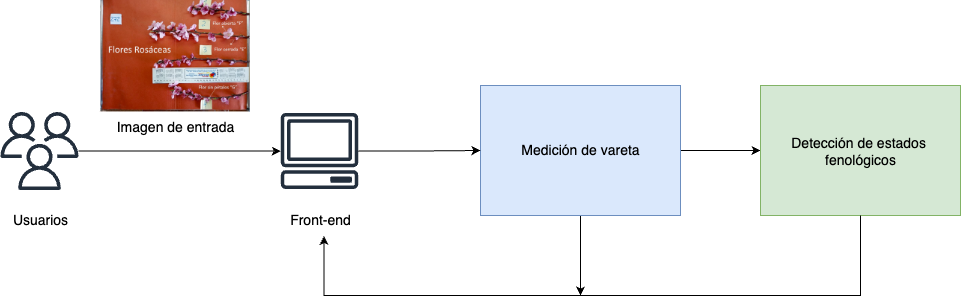
\includegraphics[scale=.4]{./Figures/arq1.drawio.png}
	\caption{Arquitectura general del sistema.}
	\label{fig:sistemaGeneral}
\end{figure}

La arquitectura del módulo que estima la longitud de la vareta se puede observar en la figura \ref{fig:varetaSize}. Este módulo toma y preprocesa la imagen de entrada, posteriormente detecta la regla que es el objeto de referencia y procede a tomar las mediciones en píxeles de dicho elemento. Luego, se hace una conversión de píxeles a centímetros. Una vez finalizada la conversión, se detectan las varetas presentes en la imagen y se calculan sus dimensiones, se revisa la orientación de la foto y se toma la longitud de cada vareta en píxeles. Finalmente, con la conversión anterior se pasa a centímetros las mediciones de las varetas, se anotan los resultados en una tabla y son enviados al siguiente módulo. Por otro lado, la imagen con las mediciones se muestra por pantalla.

Este módulo se detalla con más a profundidad en este mismo capítulo.

\begin{figure}[htpb]
	\centering
	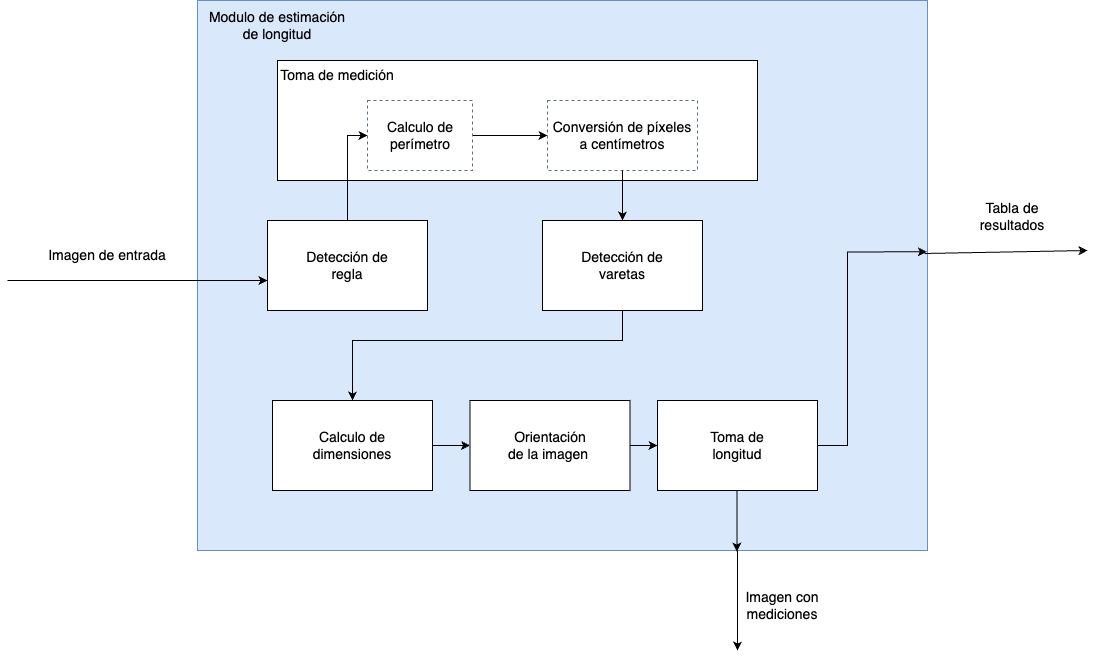
\includegraphics[scale=.4]{./Figures/medicionVareta.drawio.png}
	\caption{Módulo de estimación de longitud.}
	\label{fig:varetaSize}
\end{figure}

La arquitectura del módulo de detección y procesamiento se presenta en la figura \ref{fig:densidadDeFlores}. La entrada a este módulo es la imagen original donde se le aplica un preprocesamiento y posteriormente se pasa por un modelo que detecta los estados fenológicos de las flores de duraznero y sus varetas. Luego, se realiza un postprocesamiento de los resultados para conocer el número de flores totales que se encuentran en la imagen y un conteo de las mismas por vareta. Por último, se extraen las flores detectadas por vareta y son enviadas al clasificador para determinar su tipo.

Más adelante en este mismo capítulo se dará más información detallada de este módulo y de otros bloques del sistema que cumplen una función importante para generar los resultados deseados.

Cabe destacar que la realización de este sistema se llevó a cabo en el lenguaje de programación \textit{Python} y se encuentra diseñado para funcionar en una computadora local bajo un ambiente virtualizado. 

\begin{figure}[htp]
	\centering
	\includegraphics[scale=.35]{./Figures/DetecciónFlor.drawio.png}
	\caption{Módulo de detección y procesamiento.}
	\label{fig:densidadDeFlores}
\end{figure}

\section{Preparación de los datos}

La preparación de los datos es una de las partes más criticas durante el desarrollo de un modelo de aprendizaje. Esto debido a que si los datos no se encuentran en las condiciones adecuadas para su uso en un modelo de IA, el modelo no tendrá un buen rendimiento. 

El presente trabajo requirió la generación de distintos etiquetados para el \textit{dataset} original, debido a la cantidad de modelos utilizados durante su desarrollo.

\subsection{Análisis exploratorio}
El \textit{dataset} original provisto por el INTA contiene las características que se indican en la tabla \ref{tab:flores}. En general, las fotos presentan distintas dimensiones y orientaciones (vertical u horizontal). Por otro lado, se desconoce el tipo de cámara utilizada y el ángulo siempre es cenital.


\begin{table}[h]
	\centering
	\caption[caption corto]{Características de las fotos de duraznos}
	\begin{tabular}{c c c l}    
		\toprule
		\textbf{Formato}     & \textbf{Cantidad} & \textbf{Resolución} & \textbf{Observaciones}\\
		\midrule
		JPG                  & 286               &  Variable &  Cuatro varetas por foto.\\		
		\bottomrule
		\hline
	\end{tabular}
	\label{tab:flores}
\end{table}
 
Las imágenes tienen un fondo naranja y en ocasiones contienen partes grises. Esto debido a que las varetas de duraznero fueron posadas sobre una cartulina color naranja y a veces por las dimensiones de las varetas, se toma parte de la mesa de color gris.

Por otro lado, las fotos presentan cambios de brillo e iluminación, generando distintas tonalidades de los colores de fondo y de las flores. 

Los elementos que se observan generalmente en las fotos provistas por el cliente incluyen: una regla, cuatro varetas, una cartulina de fondo, cuatro etiquetas que identifican las varetas y en ocasiones objetos que no forman parte de la detección o que no aportan información.

En la figura \ref{fig:three graphs}, se puede observar algunos ejemplos de fotos con las características que se describieron anteriormente.

\begin{figure}[!htpb]
     \centering
     \begin{subfigure}[b]{0.4\textwidth}
         \centering
         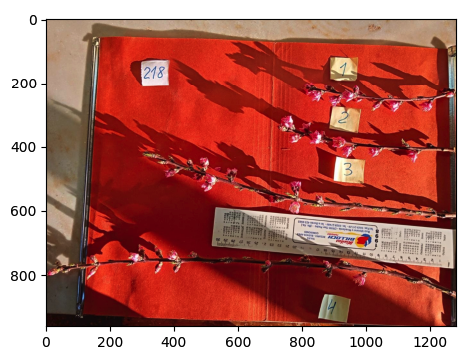
\includegraphics[scale=.4]{./Figures/flor_muestra5.png}
         \caption{Foto de muestra 1.}
         \label{fig:1de3}
     \end{subfigure}
     \hfill
     \begin{subfigure}[b]{0.4\textwidth}
         \centering
         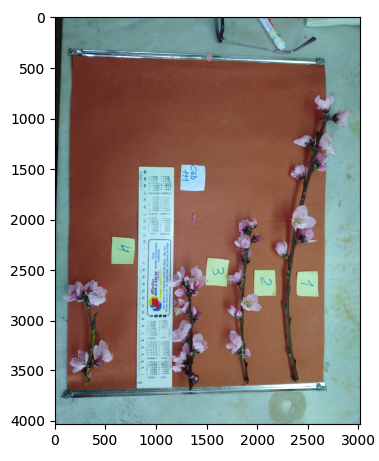
\includegraphics[scale=.4]{./Figures/flor_muestra3.png}
         \caption{Foto de muestra 2.}
         \label{fig:2de3}
     \end{subfigure}
     \hfill
     \begin{subfigure}[b]{0.5\textwidth}
         \centering
         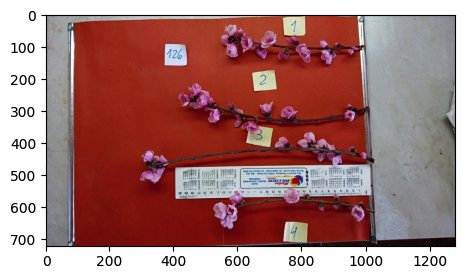
\includegraphics[scale=.45]{./Figures/flor_muestra6.png}
         \caption{Foto de muestra 3.}
         \label{fig:3de3}
     \end{subfigure}
        \caption{Fotos de muestra del conjunto de datos.}
        \label{fig:three graphs}
\end{figure}

Es importante mencionar que, las fotos de varetas tomadas por el cliente, están clasificadas por el tipo de flor que poseen las varetas. Es decir, una foto solo va a contener varetas con flores del tipo rosáceas o campanuláceas, pero no ambos tipos de flor en una misma imagen. En la figura \ref{fig:two graphs} se muestran dos fotos de varetas, una que contiene flores rosáceas y otra que contiene flores campanuláceas.

\begin{figure}[!htp]
     \centering
     \begin{subfigure}[b]{0.3\textwidth}
         \centering
         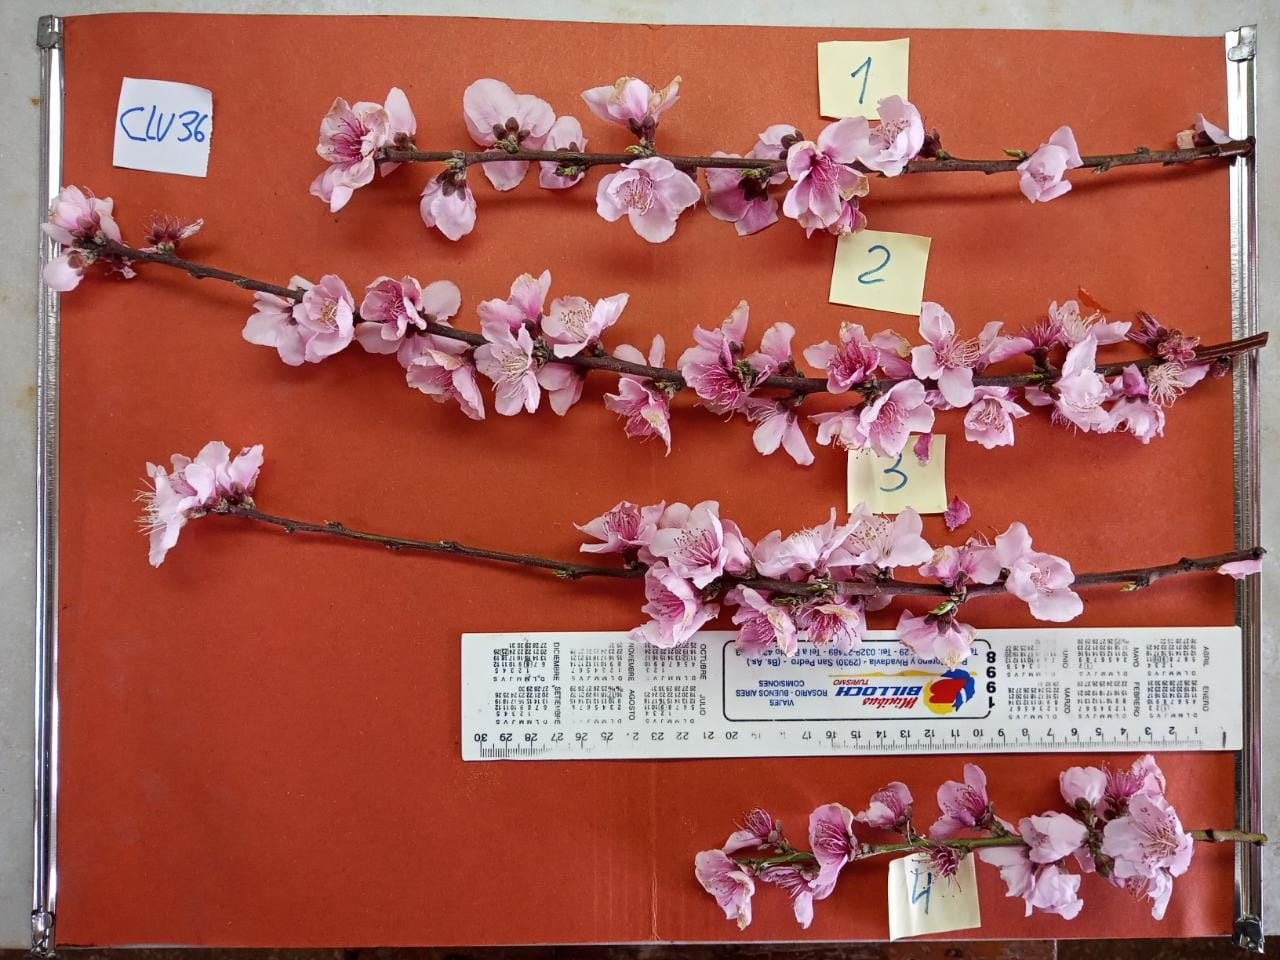
\includegraphics[scale=.15]{./Figures/flor_rosacea.jpg}
         \caption{Foto de varetas con flores rosáceas.}
         \label{fig:1de3}
     \end{subfigure}
     \hfill
     \begin{subfigure}[b]{0.4\textwidth}
         \centering
         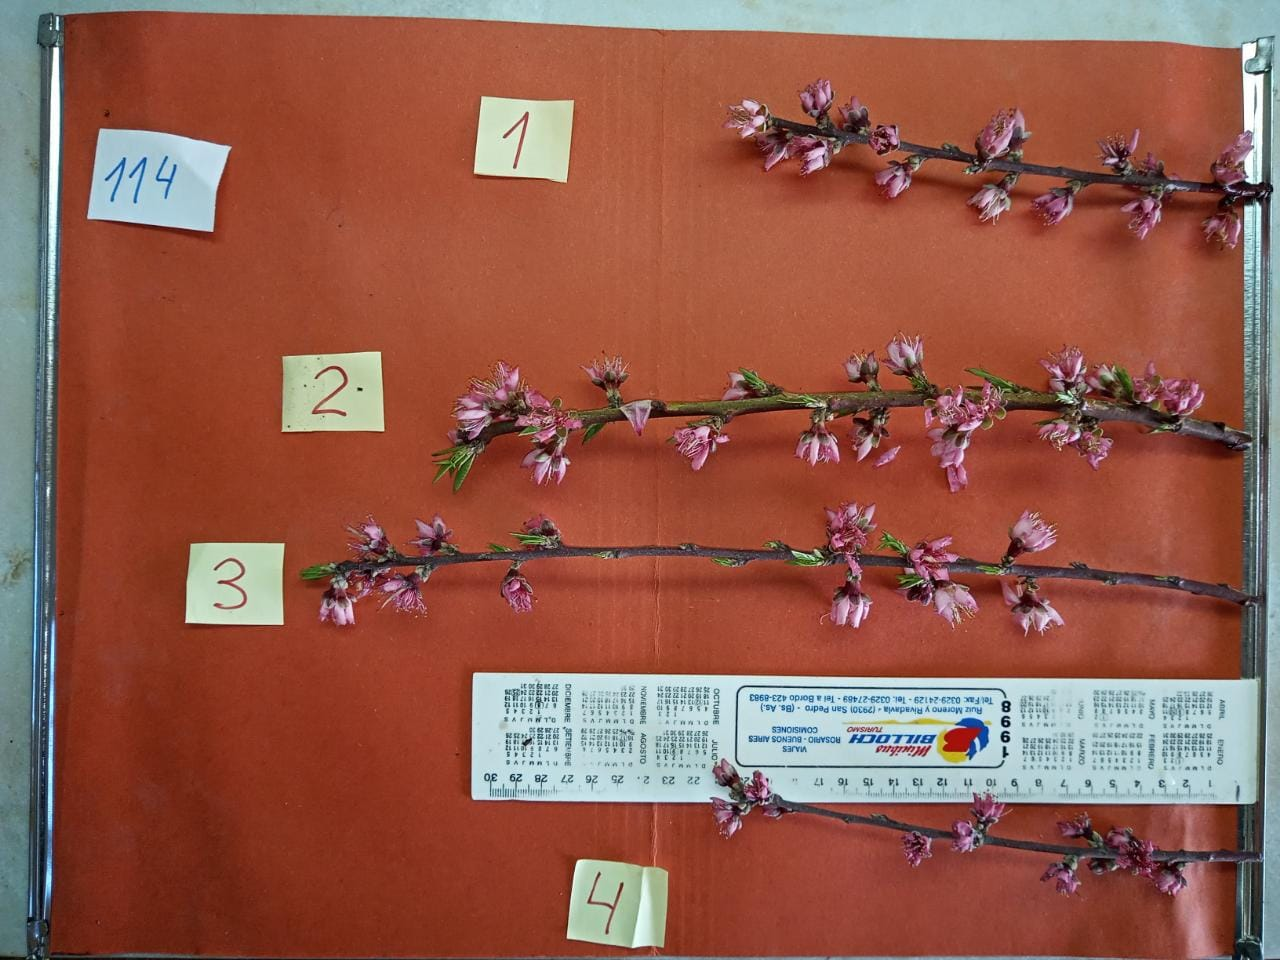
\includegraphics[scale=.15]{./Figures/flor_camp.jpg}
         \caption{Foto de varetas con flores campanuláceas.}
         \label{fig:2de3}
     \end{subfigure}
        \caption{Fotos de varetas de duraznero con su tipo flor.}
        \label{fig:two graphs}
\end{figure}

\newpage

Cabe destacar que en una foto de varetas de duraznero, se encuentran varias flores y cada flor posee un estado fenológico. Los estados fenológicos que se pueden encontrar son: flor abierta, flor cerrada y flor sin pétalos respectivamente. En la figura se observan dichos estados fenológicos para la flor de duraznero del tipo rosácea.

\subsubsection{Balanceo del \textit{dataset} antes del etiquetado}

El \textit{dataset} cuenta con un total de 286 imágenes en total, donde, 57 imágenes contienen varetas con flores del tipo campanuláceas, y 229 contienen varetas con flores del tipo rosáceas. Por lo tanto, se considera que el conjunto de datos se encuentra desbalanceado con respecto al tipo de flor. 




 
%\definecolor{mygreen}{rgb}{0,0.6,0}
%\definecolor{mygray}{rgb}{0.5,0.5,0.5}
%\definecolor{mymauve}{rgb}{0.58,0,0.82}
%
%%%%%%%%%%%%%%%%%%%%%%%%%%%%%%%%%%%%%%%%%%%%%%%%%%%%%%%%%%%%%%%%%%%%%%%%%%%%%%
%% parámetros para configurar el formato del código en los entornos lstlisting
%%%%%%%%%%%%%%%%%%%%%%%%%%%%%%%%%%%%%%%%%%%%%%%%%%%%%%%%%%%%%%%%%%%%%%%%%%%%%%
%\lstset{ %
%  backgroundcolor=\color{white},   % choose the background color; you must add \usepackage{color} or \usepackage{xcolor}
%  basicstyle=\footnotesize,        % the size of the fonts that are used for the code
%  breakatwhitespace=false,         % sets if automatic breaks should only happen at whitespace
%  breaklines=true,                 % sets automatic line breaking
%  captionpos=b,                    % sets the caption-position to bottom
%  commentstyle=\color{mygreen},    % comment style
%  deletekeywords={...},            % if you want to delete keywords from the given language
%  %escapeinside={\%*}{*)},          % if you want to add LaTeX within your code
%  %extendedchars=true,              % lets you use non-ASCII characters; for 8-bits encodings only, does not work with UTF-8
%  %frame=single,	                % adds a frame around the code
%  keepspaces=true,                 % keeps spaces in text, useful for keeping indentation of code (possibly needs columns=flexible)
%  keywordstyle=\color{blue},       % keyword style
%  language=[ANSI]C,                % the language of the code
%  %otherkeywords={*,...},           % if you want to add more keywords to the set
%  numbers=left,                    % where to put the line-numbers; possible values are (none, left, right)
%  numbersep=5pt,                   % how far the line-numbers are from the code
%  numberstyle=\tiny\color{mygray}, % the style that is used for the line-numbers
%  rulecolor=\color{black},         % if not set, the frame-color may be changed on line-breaks within not-black text (e.g. comments (green here))
%  showspaces=false,                % show spaces everywhere adding particular underscores; it overrides 'showstringspaces'
%  showstringspaces=false,          % underline spaces within strings only
%  showtabs=false,                  % show tabs within strings adding particular underscores
%  stepnumber=1,                    % the step between two line-numbers. If it's 1, each line will be numbered
%  stringstyle=\color{mymauve},     % string literal style
%  tabsize=2,	                   % sets default tabsize to 2 spaces
%  title=\lstname,                  % show the filename of files included with \lstinputlisting; also try caption instead of title
%  morecomment=[s]{/*}{*/}
%}
%
%
%%----------------------------------------------------------------------------------------
%%	SECTION 1
%%----------------------------------------------------------------------------------------
%\section{Análisis del software}
% 
%La idea de esta sección es resaltar los problemas encontrados, los criterios utilizados y la justificación de las decisiones que se hayan tomado.
%
%Se puede agregar código o pseudocódigo dentro de un entorno lstlisting con el siguiente código:
%
%\begin{verbatim}
%\begin{lstlisting}[caption= "un epígrafe descriptivo"]
%	las líneas de código irían aquí...
%\end{lstlisting}
%\end{verbatim}
%
%A modo de ejemplo:
%
%\begin{lstlisting}[label=cod:vControl,caption=Pseudocódigo del lazo principal de control.]  % Start your code-block
%
%#define MAX_SENSOR_NUMBER 3
%#define MAX_ALARM_NUMBER  6
%#define MAX_ACTUATOR_NUMBER 6
%
%uint32_t sensorValue[MAX_SENSOR_NUMBER];		
%FunctionalState alarmControl[MAX_ALARM_NUMBER];	//ENABLE or DISABLE
%state_t alarmState[MAX_ALARM_NUMBER];						//ON or OFF
%state_t actuatorState[MAX_ACTUATOR_NUMBER];			//ON or OFF
%
%void vControl() {
%
%	initGlobalVariables();
%	
%	period = 500 ms;
%		
%	while(1) {
%
%		ticks = xTaskGetTickCount();
%		
%		updateSensors();
%		
%		updateAlarms();
%		
%		controlActuators();
%		
%		vTaskDelayUntil(&ticks, period);
%	}
%}
%\end{lstlisting}




	% Chapter Template

\chapter{Ensayos y resultados} % Main chapter title

\label{Chapter4} % Change X to a consecutive number; for referencing this chapter elsewhere, use \ref{ChapterX}

%----------------------------------------------------------------------------------------
%	SECTION 1
%----------------------------------------------------------------------------------------
En este capítulo se describen los ensayos realizados y se presentan y comparan los resultados obtenidos.

\section{Banco de pruebas}
\label{sec:pruebasHW}

Para el desarrollo del presente proyecto se utilizaron 3 bancos de pruebas, con las siguientes especificaciones técnicas:

\begin{itemize}
\item Banco de pruebas \textit{Laptop} \textit{MacBook Pro} - \textit{hardware} disponible:
	\begin{itemize}
	\item \textbf{OS}: \textit{MacOS Sonoma} 14.
	\item \textbf{CPU}: Apple M1 Pro.
	\item \textbf{RAM}: 32 GB.
	\item \textbf{GPU}: No contiene.
	\end{itemize}
\item Banco de pruebas \textit{Laptop} \textit{ASUS TUF GAMING F15} - \textit{hardware} disponible:
	\begin{itemize}
	\item \textbf{OS}: \textit{Windows} 11.
	\item \textbf{CPU}: \textit{Intel(R) Core(TM)} i5-11260H.
	\item \textbf{RAM}: 16 GB.
	\item \textbf{GPU}: \textit{NVIDIA GeForce RTX} 3050.
	\end{itemize}
\item Banco de pruebas \textit{Google Colab Pro} - \textit{hardware} disponible:
	\begin{itemize}
	\item \textbf{OS}: desconocido.
	\item \textbf{CPU}: desconocido.
	\item \textbf{RAM}: 12,5 GB.
	\item \textbf{GPU}: T4.
	\end{itemize}
\end{itemize}

\section{Desempeño de modelos}
\label{sec:desempeñoMod}

Para medir el desempeño de los modelos de AI utilizados durante la ejecución de este proyecto, se decidió emplear la métrica \textit{mAP}. Esta métrica evalúa tanto la clasificación del objeto como la ubicación del \textit{bounding box} a través del \textit{Avarage Precision} (\textit{AP}) que se representa en la ecuación \ref{eq:AP}.

\begin{equation}
    \label{eq:AP}
    \text{AP} = \frac{1}{n} \sum_{k=1}^n \text{Precisión en } k \times \text{Rel}_{k}
\end{equation}

Siendo
\begin{itemize}
    \item \( n \) el número total de elementos recuperados.
    \item \(\text{Precision at } k\) la precisión en el \( k \)-ésimo punto de recuperación.
    \item \(\text{Rel}_{k}\) un indicador binario que denota si el elemento en el \( k \)-ésimo punto de recuperación es relevante (\( \text{Rel}_{k} = 1 \)) o no relevante (\( \text{Rel}_{k} = 0 \)).
\end{itemize}

Luego, al promediar los valores de \textit{AP} entre todas las clases, se obtiene respectivamente el \textit{mAP} y la ecuación quedaría como se muestra en \ref{eq:mAP}.

\begin{equation}
    \label{eq:mAP}
    \text{mAP} = \frac{1}{C} \sum_{c=1}^C \text{AP}_c
\end{equation}

Donde 
\begin{itemize}
	\item \( C \) es el número total de clases o consultas.
    \item \( AP \) es el Average Precision calculado para la clase o consulta.
\end{itemize}

\subsection{Desempeño del detector de regla}

El detector de la regla como se mencionó en el capítulo anterior,  tiene como modelo base un \textit{YOLOv8n} y cumple una función fundamental para la estimación de la longitud de la vareta. Por otro lado, el entrenamiento de este modelo se realizó con los siguientes hiperparámetros:

\begin{itemize}
	\item Epocas: 100.
    \item Tamaño de imagen de entrada: 640 x 640.
    \item \textit{Batch}: 16.
    \item \textit{Learning rate}: 0.01.
\end{itemize}

Los resultados obtenidos para la detección de este elemento contra el conjunto de datos de prueba se observan en la tabla \ref{tab:resultadosRegla}.

\begin{table}[h]
	\centering
	\caption{Métricas de detección para el detector de regla.}
	\begin{tabular}{c c c c c c c}    
		\toprule
		\textbf{Clase}&\textbf{Imágenes}&\textbf{Objetos encontrados}&\textbf{Precision} &\textbf{Recall}&\textbf{mAP 50}&\textbf{mAP 50-95}\\
		\midrule
		Regla & 13 & 13 & 0.996 & 1.0 & 0.995 & 0.995\\		
		\bottomrule
		\hline
	\end{tabular}
	\label{tab:resultadosRegla}
\end{table}

Los resultados fueron muy buenos en general. El modelo puede detectar la regla sin dificultad en el 99\% de los casos.

\subsection{Desempeño del detector de vareta}

El detector de vareta destinado para el módulo de estimación de longitud, tiene como modelo base un \textit{YOLOv8n} entrenado bajo los siguientes hiperparámetros:

\begin{itemize}
	\item Epocas: 100.
    \item Tamaño de imagen de entrada: 640 x 640.
    \item \textit{Batch}: 16.
    \item \textit{Learning rate}: 0.01.
\end{itemize}

Para este modelo se hicieron dos prubas, una sin aumento de datos y otra con aumento. El aumento de datos aplicado se describe en la sección \ref{aumentoDatos}.

Los resultados obtenidos contra el conjunto de datos de pruebas para el modelo sin aumento de datos se muestran en la tabla \ref{tab:resultadosVareta}.

\begin{table}[h]
	\centering
	\caption{Métricas de detección para el detector de varetas sin aumento de datos.}
	\begin{tabular}{c c c c c c c}    
		\toprule
		\textbf{Clase}&\textbf{Imágenes}&\textbf{Objetos encontrados}&\textbf{Precision} &\textbf{Recall}&\textbf{mAP 50}&\textbf{mAP 50-95}\\
		\midrule
		Vareta & 10 & 40 & 1.0 & 0.923 & 0.983 & 0.574\\		
		\bottomrule
		\hline
	\end{tabular}
	\label{tab:resultadosVareta}
\end{table}

Como se puede observar, el modelo sin aumento de datos, consigue detectar un total de 40 varetas en 10 imágenes, donde todas las detecciones fueron correctas. Por otro lado, el modelo logra una precisión promedio de detección del 98.3\% cuando se requiere un nivel de confianza igual al 50\%, pero el \textit{mAP} 50-95, indica que en los casos donde el nivel de confianza esta entre el 50\% y 95\%, la precisión promedio, es de un 57.4\%. Por este motivo, se decidió aplicar aumento de datos.

Los resultados con aumento de datos se pueden observar en la tabla \ref{tab:resultadosVaretaConAug}.

\begin{table}[h]
	\centering
	\caption{Métricas de detección para el detector de varetas con aumento de datos.}
	\begin{tabular}{c c c c c c c}    
		\toprule
		\textbf{Clase}&\textbf{Imágenes}&\textbf{Objetos encontrados}&\textbf{Precision} &\textbf{Recall}&\textbf{mAP 50}&\textbf{mAP 50-95}\\
		\midrule
		Vareta & 10 & 40 & 0.974 & 0.975 & 0.976 & 0.702\\		
		\bottomrule
		\hline
	\end{tabular}
	\label{tab:resultadosVaretaConAug}
\end{table}

Luego de aplicar aumento de datos, se observa que, el modelo mejoró la cantidad de veces donde detecta de forma precisa a la clase vareta en un 5.2\% con respecto al modelo sin aumento de datos. Por otro lado, también se incrementó la precisión promedio al 70.2\% cuando se tiene un umbral de confianza que va entre 50\% y 95\%.

Con esto se destaca que, el aumento de datos mejoró el rendimiento del modelo de forma considerable.

\subsection{Desempeño del detector de estados fenológicos}

La detección de estados fenológicos, como se mencionó en el capítulo anterior, fue probada con dos modelos de IA que se ajustan para este caso de uso. Por un lado, se probó con un detector de dos etapas como es \textit{Faster R-CNN} y por otro lado con un detector de una etapa como \textit{YOLOv8}. Ambos casos, se probaron con y sin el uso de aumento de datos. Los resultados fueron los siguientes:

\subsubsection{\textit{Faster R-CNN} sin aumento de datos}

El entrenamiento del modelo se hizo bajo los siguientes hiperparámentros:

\begin{itemize}
	\item Epocas: 100.
    \item Tamaño de imagen de entrada: 640 x 640.
    \item \textit{Batch}: 4.
    \item \textit{Learning rate}: 0.001.
    \item \textit{Momentum}: 0.9.
    \item \textit{Weight decay}: 0.0005.
    \item \textit{Optimizer}: \textit{Stochastic gradient descent}.
\end{itemize}

Los resultados de detección contra el conjunto de prueba se muestra en la tabla \ref{tab:resultadosFasterSinAug}.

\begin{table}[h]
	\centering
	\caption{Métricas de detección para \textit{Faster R-CNN} sin aumento de datos.}
	\begin{tabular}{c c c c c c c}    
		\toprule
		\textbf{Clase}&\textbf{Imágenes}&\textbf{mAP}&\textbf{mAP 50}&\textbf{mAP > 50}\\
		\midrule
		Todas & 14 & 0.3492 & 0.5970 & 0.3605\\
		Flor abierta & 14 & 0.4313 & - & - \\
		Flor cerrada & 14 & 0.1525 & - & - \\
		Flor sin pétalos & 14 & 0.3735 & - & - \\
		Incierto & 14 & 0.0942 & - & - \\
		Vareta & 14 & 0.6947 & - & - \\		
		\bottomrule
		\hline
	\end{tabular}
	\label{tab:resultadosFasterSinAug}
\end{table}

La precisión promedio de detección entre todas las clases es de un 34.9\%, lo que significa que, el modelo tiene una precisión del 34.9\% al detectar las diferentes clases en el conjunto de datos. Además, El modelo logra una precisión de detección del 59.7\% cuando se considera un umbral de confianza igual al 50\% y para detecciones con un nivel de confianza mayor al 50\% se tiene una precisión del 36.1\%.

Por otro lado, al evaluar la precisión promedio de detección por clase, se observa que la categoría \textit{vareta}, es la clase a la que el modelo detecta con mejor precisión promedio con 69.5\%, seguida por \textit{flor abierta} con 43.13\% y por \textit{flor sin pétalos} con 37.35\%. Además, se muestra que el modelo detecta con dificultad las categorías \textit{flor cerrada} con un \textit{mAP} de 12.25\% e \textit{incierto} con 9.42\%.

Este bajo porcentaje de \textit{mAP} para la clase \textit{flor cerrada} con respecto a las otras categorías presentes, se puede deber al desbalance de datos observado en la sección \ref{desbalanceAfterLabeled} y al rendimiento del modelo al intentar detectar objetos pequeños en la imagen. Adicionalmente, para la categoría \textit{incierto} no se cuenta con una cantidad de muestras significativas y consistente a través del conjunto de datos, lo que explica la baja precisión promedio obtenida para esta clase.

Para mejorar estos resultados se implementó el aumento de datos mencionado en la sección \ref{aumentoDatos}.

\subsubsection{\textit{Faster R-CNN} con aumento de datos}

El rendimiento del modelo basado en la métrica \textit{mAP}, se puede observar en la tabla \ref{tab:resultadosFasterConAug}. 

\begin{table}[h]
	\centering
	\caption{Métricas de detección para \textit{Faster R-CNN} con aumento de datos.}
	\begin{tabular}{c c c c c c c}    
		\toprule
		\textbf{Clase}&\textbf{Imágenes}&\textbf{mAP}&\textbf{mAP 50}&\textbf{mAP > 50}\\
		\midrule
		Todas & 14 & 0.3733 & 0.6328 & 0.3793\\
		Flor abierta & 14 & 0.5143 & - & - \\
		Flor cerrada & 14 & 0.2049 & - & - \\
		Flor sin pétalos & 14 & 0.3290 & - & - \\
		Incierto & 14 & 0.0887 & - & - \\
		Vareta & 14 & 0.7294 & - & - \\		
		\bottomrule
		\hline
	\end{tabular}
	\label{tab:resultadosFasterConAug}
\end{table}
\newpage
Como se puede observar, se logra mejorar la precisión promedio de detección para las clases \textit{flor abierta}, \textit{flor cerrada} y \textit{vareta}. Con esto, la métrica \textit{mAP} medida entre todas las clases mejora a 37.33\%, adicionalmente también aumenta a 63.26\% cuando se fija un umbral de confianza de detección igual al 50\% y a un 37.93\% cuando el nivel de confianza en la detección es superior al 50\%.

Se puede concluir que el modelo \textit{Faster R-CNN} con y sin aumento de datos es bueno para detectar la vareta y las flores en estado abierto. Este comportamiento se puede deber al tamaño de estos objetos en la imagen en comparación con el resto de las categorías que se busca en la detección. Además, la clase \textit{flor abierta} es la clase más predominante en todas las imágenes según el estudio de los datos realizado en la sección \ref{desbalanceAfterLabeled}, lo que permite que el modelo pueda aprender y reconocer con mayor precisión sus características debido a la abundancia de ejemplos representativos durante el entrenamiento.

\subsubsection{\textit{YOLOv8n} sin aumento de datos}

El resultado obtenido con \textit{YOLOv8n} sin aumento de datos, con 14 imágenes del conjunto de pruebas y bajo los siguientes parámetros de entrenamiento:

\begin{itemize}
	\item Epocas: 100.
    \item Tamaño de imagen de entrada: 640 x 640.
    \item \textit{Batch}: 16.
    \item \textit{Learning rate}: 0.01.
\end{itemize}

Se puede observar en la tabla \ref{tab:resultadosYoloSinAug}.

\begin{table}[h]
	\centering
	\caption{Métricas de detección para \textit{YOLOv8n} sin aumento de datos.}
	\begin{tabular}{c c c c c c c}    
		\toprule
		\textbf{Clase}&\textbf{Imágenes}&\textbf{mAP 50}&\textbf{mAP > 50}\\
		\midrule
		Todas & 14 & 0.645 & 0.418\\
		Flor abierta & 14 & 0.905 & 0.611 \\
		Flor cerrada & 14 & 0.614 & 0.251 \\
		Flor sin pétalos & 14 & 0.588 & 0.363 \\
		Incierto & 14 & 0.122 & 0.065 \\
		Vareta & 14 & 0.994 & 0.802 \\		
		\bottomrule
		\hline
	\end{tabular}
	\label{tab:resultadosYoloSinAug}
\end{table}

Se puede observar que \textit{YOLOv8n} tiene una precisión promedio, entre todas las clases, cuando se fija un umbral del 50\% de 64.5\%, que supera al \textit{mAP} 50 obtenido con el modelo \textit{Faster R-CNN} con y sin aumento de datos.

Las clases que este modelo detecta con más precisión son: vareta, flor abierta y flor cerrada. La diferencia y mejora contra \textit{Faster R-CNN} se puede observar también al comparar la métrica \textit{mAP} obtenida para todas las clases donde este modelo se desempeño mejor. Como ejemplo se tiene la clase \textit{vareta} donde se obtuvo un 69.5\% y, con \textit{YOLOv8n}, esta misma clase que también fue la mejor para este modelo tuvo 99.4\% que representa una mejora del 29.9\%.

Por otro lado la clase \textit{vareta}, en general, ambos modelos la logran detectar con alta precisión y esto se puede deber al tamaño de este objeto en la imagen. Además, es seguida por la clase \textit{flor abierta} que, como se mencionó anteriormente, contiene una cantidad de muestras representativas que ayudan al modelo a reconocer los patrones de esta clase. Por último, se destaca la categoría \textit{incierto}, que tanto este modelo como \textit{Faster R-CNN} no logran reconocer durante la detección en su totalidad.

La matriz de confusión normalizada mostrada en la figura \ref{fig:cfmatriznorm}, indica que muchas de las veces que se tiene la clase \textit{incierto}, el modelo la predice como \textit{flor abierta}. Lo que demuestra que el modelo durante el entrenamiento no logró aprender correctamente los patrones que identifican dicha clase.

\begin{figure}[ht]
	\centering
	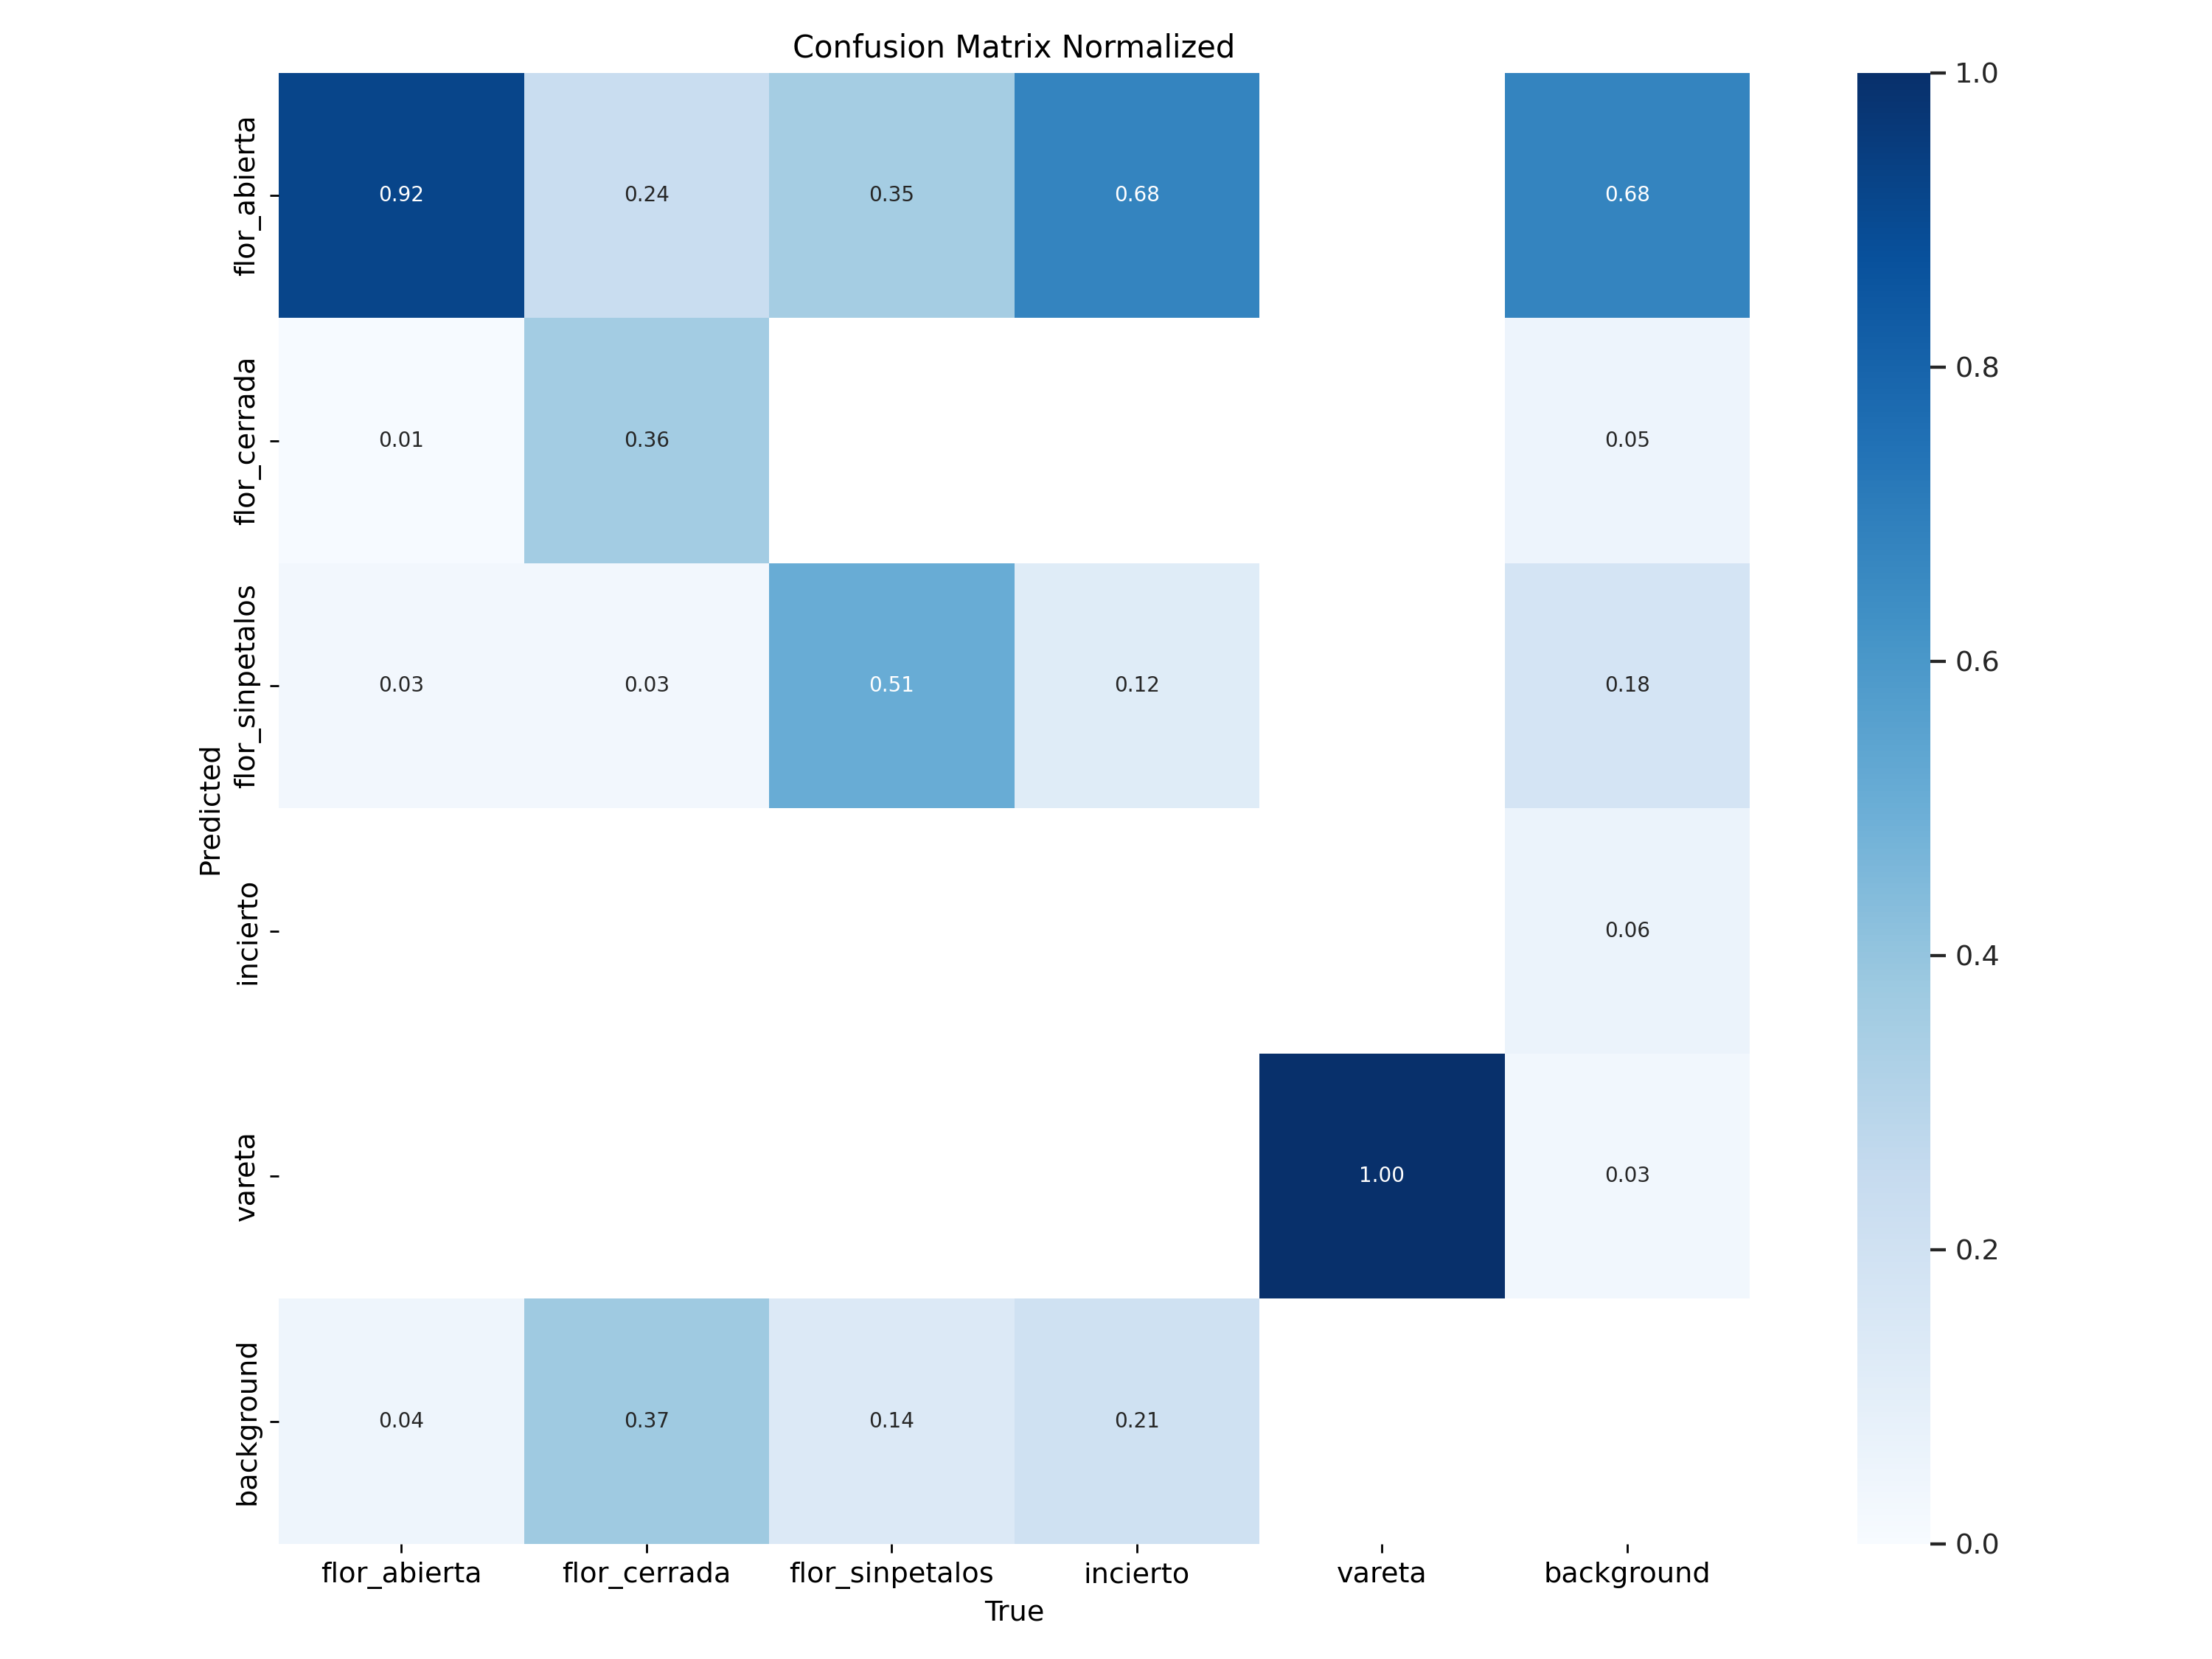
\includegraphics[scale=0.52]{./Figures/CFMatrixnorm.png}
	\caption{Matriz de confusión normalizada de \textit{YOLOv8n} para el conjunto de prueba.}
	\label{fig:cfmatriznorm}
\end{figure}

\subsubsection{\textit{YOLOv8n} con aumento de datos}

Para mejorar los resultados de \textit{YOLOv8n} se implementó el aumento de datos descrito en la sección \ref{aumentoDatos}. Los resultados obtenidos contra el conjunto de imágenes de prueba, se observa en la tabla \ref{tab:resultadosYoloConAug}.

\begin{table}[h]
	\centering
	\caption{Métricas de detección para \textit{YOLOv8n} con aumento de datos.}
	\begin{tabular}{c c c c c c c}    
		\toprule
		\textbf{Clase}&\textbf{Imágenes}&\textbf{mAP 50}&\textbf{mAP > 50}\\
		\midrule
		Todas & 14 & 0.655 & 0.423\\
		Flor abierta & 14 & 0.893 & 0.611 \\
		Flor cerrada & 14 & 0.673 & 0.266 \\
		Flor sin pétalos & 14 & 0.603 & 0.373 \\
		Incierto & 14 & 0.111 & 0.065 \\
		Vareta & 14 & 0.995 & 0.802 \\		
		\bottomrule
		\hline
	\end{tabular}
	\label{tab:resultadosYoloConAug}
\end{table}

La precisión promedio para un umbral de confianza igual al 50\% mejora para la clase \textit{flor cerrada} en un 5.9\% , para la clase \textit{flor sin pétalos} en un 1.5\%. Mientras que se tiene una perdida para la clase flor abierta del 1.2\%. Quedando el \textit{mAP} 50 entre todas las clases con un aumento del 1\%.

Se observa que el entrenamiento del modelo con aumento de datos ayudó a mejorar el reconocimiento de las clases más difíciles de detectar como son \textit{flor cerrada} y \textit{flor sin pétalos}. Además, mantiene el buen rendimiento para las clases \textit{flor abierta} y \textit{vareta}.

Al comparar todos los experimentos realizados para la detección de los estados fenológicos de las flores de duraznero, el modelo con mejor rendimiento basado en la métrica \textit{mAP} para dicha tarea es \textit{YOLOv8n} con aumento de datos. Por este motivo, se seleccionó este modelo para desempeñar dicha tarea.

Por último, se aplicó \textit{Eigen-CAM} \cite{ARTICLE:17} para crear mapas de calor que permitan explicar los resultados obtenidos por el modelo. Este mapa de calor se implementó en la capa convolucional \textit{C2f}. En la figura \ref{fig:EigenCam}, se observa un ejemplo de los mapas de calor generados por \textit{Eigen-CAM} en una foto perteneciente al conjunto de pruebas utilizando \textit{YOLOv8n} con aumento de datos.

\begin{figure}[ht]
	\centering
	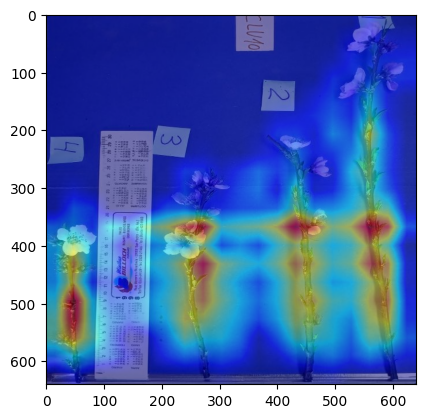
\includegraphics[scale=0.55]{./Figures/EigenCamEj.png}
	\caption{Mapa de calor con \textit{Eigen-CAM} en la capa \textit{C2f} del modelo \textit{YOLOv8n}.}
	\label{fig:EigenCam}
\end{figure}
\newpage

Se observa que los mapas de activación están enfocados en las varetas para la capa convolucional seleccionada, lo que sugiere que el modelo pone mayor atención en este objeto al momento de realizar la detección.   

\section{Desempeño de módulos}
\label{sec:desempeñoModulos}

El sistema como se mencionó en secciones anteriores, cuenta con dos módulos, y para estimar su desempeño se utiliza un método visual. Este método implica la introducción de una imagen o fotografía en el sistema, permitiendo que esta transite a través de cada módulo de manera secuencial. Posteriormente, se realiza una observación de la salida generada por cada módulo de forma individual y se toman conclusiones de su funcionamiento. Esta aproximación no solo facilita la medición del rendimiento del sistema en su totalidad, sino que también permite un examen detallado de las contribuciones y funcionalidades específicas de cada uno de sus componentes modulares.

\subsection{Desempeño del módulo de estimación de longitud} 
	% Chapter Template

\chapter{Conclusiones} % Main chapter title

\label{Chapter5} % Change X to a consecutive number; for referencing this chapter elsewhere, use \ref{ChapterX}


%----------------------------------------------------------------------------------------

%----------------------------------------------------------------------------------------
%	SECTION 1
%----------------------------------------------------------------------------------------

En este capítulo se presenta las conclusiones del trabajo en general, los principales aportes obtenidos y los próximos pasos.

\section{Conclusiones generales }



%La idea de esta sección es resaltar cuáles son los principales aportes del trabajo realizado y cómo se podría continuar. Debe ser especialmente breve y concisa. Es buena idea usar un listado para enumerar los logros obtenidos.
%
%Algunas preguntas que pueden servir para completar este capítulo:
%
%\begin{itemize}
%\item ¿Cuál es el grado de cumplimiento de los requerimientos?
%\item ¿Cuán fielmente se puedo seguir la planificación original (cronograma incluido)?
%\item ¿Se manifestó algunos de los riesgos identificados en la planificación? ¿Fue efectivo el plan de mitigación? ¿Se debió aplicar alguna otra acción no contemplada previamente?
%\item Si se debieron hacer modificaciones a lo planificado ¿Cuáles fueron las causas y los efectos?
%\item ¿Qué técnicas resultaron útiles para el desarrollo del proyecto y cuáles no tanto?
%\end{itemize}


%----------------------------------------------------------------------------------------
%	SECTION 2
%----------------------------------------------------------------------------------------
\section{Próximos pasos}

Acá se indica cómo se podría continuar el trabajo más adelante.
 
\end{verbatim}

Los apéndices también deben escribirse en archivos .tex separados, que se deben ubicar dentro de la carpeta \emph{Appendices}. Los apéndices vienen comentados por defecto con el caracter \code{\%} y para incluirlos simplemente se debe eliminar dicho caracter.

Finalmente, se encuentra el código para incluir la bibliografía en el documento final.  Este código tampoco debe modificarse. La metodología para trabajar las referencias bibliográficas se desarrolla en la sección \ref{sec:biblio}.
%----------------------------------------------------------------------------------------

\section{Bibliografía}
\label{sec:biblio}

Las opciones de formato de la bibliografía se controlan a través del paquete de latex \option{biblatex} que se incluye en la memoria en el archivo memoria.tex.  Estas opciones determinan cómo se generan las citas bibliográficas en el cuerpo del documento y cómo se genera la bibliografía al final de la memoria.

En el preámbulo se puede encontrar el código que incluye el paquete biblatex, que no requiere ninguna modificación del usuario de la plantilla, y que contiene las siguientes opciones:

\begin{lstlisting}
\usepackage[backend=bibtex,
	natbib=true, 
	style=numeric, 
	sorting=none]
{biblatex}
\end{lstlisting}

En el archivo \file{reference.bib} se encuentran las referencias bibliográficas que se pueden citar en el documento.  Para incorporar una nueva cita al documento lo primero es agregarla en este archivo con todos los campos necesario.  Todas las entradas bibliográficas comienzan con $@$ y una palabra que define el formato de la entrada.  Para cada formato existen campos obligatorios que deben completarse. No importa el orden en que las entradas estén definidas en el archivo .bib.  Tampoco es importante el orden en que estén definidos los campos de una entrada bibliográfica. A continuación se muestran algunos ejemplos:

\begin{lstlisting}
@ARTICLE{ARTICLE:1,
    AUTHOR="John Doe",
    TITLE="Title",
    JOURNAL="Journal",
    YEAR="2017",
}
\end{lstlisting}


\begin{lstlisting}
@BOOK{BOOK:1,
    AUTHOR="John Doe",
    TITLE="The Book without Title",
    PUBLISHER="Dummy Publisher",
    YEAR="2100",
}
\end{lstlisting}


\begin{lstlisting}
@INBOOK{BOOK:2,
    AUTHOR="John Doe",
    TITLE="The Book without Title",
    PUBLISHER="Dummy Publisher",
    YEAR="2100",
    PAGES="100-200",
}
\end{lstlisting}


\begin{lstlisting}
@MISC{WEBSITE:1,
    HOWPUBLISHED = "\url{http://example.com}",
    AUTHOR = "Intel",
    TITLE = "Example Website",
    MONTH = "12",
    YEAR = "1988",
    URLDATE = {2012-11-26}
}
\end{lstlisting}

Se debe notar que los nombres \emph{ARTICLE:1}, \emph{BOOK:1}, \emph{BOOK:2} y \emph{WEBSITE:1} son nombres de fantasía que le sirve al autor del documento para identificar la entrada. En este sentido, se podrían reemplazar por cualquier otro nombre.  Tampoco es necesario poner : seguido de un número, en los ejemplos sólo se incluye como un posible estilo para identificar las entradas.

La entradas se citan en el documento con el comando: 

\begin{verbatim}
\citep{nombre_de_la_entrada}
\end{verbatim}

Y cuando se usan, se muestran así: \citep{ARTICLE:1}, \citep{BOOK:1}, \citep{BOOK:2}, \citep{WEBSITE:1}.  Notar cómo se conforma la sección Bibliografía al final del documento.

Finalmente y como se mencionó en la subsección \ref{subsec:configurando}, para actualizar las referencias bibliográficas tanto en la sección bibliografía como las citas en el cuerpo del documento, se deben ejecutar las herramientas de compilación PDFLaTeX, BibTeX, PDFLaTeX, PDFLaTeX, en ese orden.  Este procedimiento debería resolver cualquier mensaje "Citation xxxxx on page x undefined".
